\documentclass[12pt]{book}
\usepackage{t1enc} %betűkódolás
\usepackage[utf8]{inputenc} %kódolás
\usepackage[english, magyar]{babel} %nyelv
\usepackage{amsmath, amssymb, amsfonts, amsthm} %thm: tételek, definíciók
\usepackage{xcolor} %színek
\usepackage{graphicx} %grafika beillesztéséhez szükséges csomag
\usepackage{geometry} %oldalbeállítás:
\geometry{a4paper, left=25mm, right=25mm, bottom=25mm, top=25mm, footskip=10mm} %footskip: élőláb és szöveg távolsága
\usepackage[mathcal]{euscript}

\usepackage{enumitem} %számozott listákhoz kell, beállítások:
\setlist[enumerate,1]{label=\textbf{\arabic*.},itemsep=1pt,topsep=0pt,align=right}
\setlist[enumerate,2]{label=\textit{\alph*)},itemsep=1pt,topsep=0pt,align=right}

\usepackage[unicode, breaklinks]{hyperref} %hivatkozások
\hypersetup
{
	colorlinks = true,
	citecolor  = gray,
	urlcolor   = blue,
	linkcolor  = black
}

%Tétel-típus definíciók:
\theoremstyle{plain} %vastag betűs címke, dőlt betűs szöveg
\newtheorem{fa}{Feladat}[section] %szakasz megjelenése a számozásban
\theoremstyle{definition} %vastag betűs címke, álló betűs szöveg
\newtheorem{defi/}{Definíció}[section]
\newenvironment{defi}
  {\renewcommand{\qedsymbol}{$\clubsuit$}%
   \pushQED{\qed}\begin{defi/}}
  {\popQED\end{defi/}}
\newtheorem{lem/}{Lemma}[section]
\newenvironment{lem}
  {\renewcommand{\qedsymbol}{$\clubsuit$}%
   \pushQED{\qed}\begin{lem/}}
  {\popQED\end{lem/}}
\newtheorem{all/}{Állítás}[section]
\newenvironment{all}
{\renewcommand{\qedsymbol}{$\clubsuit$}%
	\pushQED{\qed}\begin{all/}}
	{\popQED\end{all/}}
\newtheorem{pl}{Példa}[section]
\newtheorem{theo/}{Tétel}[section]
\newenvironment{theo}
  {\renewcommand{\qedsymbol}{$\clubsuit$}%
   \pushQED{\qed}\begin{theo/}}
  {\popQED\end{theo/}}
\theoremstyle{remark}
\newtheorem*{mj}{Megjegyzés}

\parindent=0mm
\parskip=3mm
\frenchspacing

%Saját egyéb csomagok:
\usepackage{gensymb} %\degree fok parancs
\usepackage{mathtools} %\coloneqq :=
\usepackage{fancyhdr} %élőfej, élőláb
\usepackage{comment} %többsoros komment
\usepackage{array}

%???
\usepackage{mathptmx}
\usepackage[stable]{footmisc}
\usepackage{multirow}
\usepackage{colortbl}
\usepackage{ragged2e}

%Egyéb definíciók:
\renewcommand\qedsymbol{$\blacksquare$}
\newcommand\tg{\operatorname{tg}}
\newcommand\ctg{\operatorname{ctg}}
\newcommand\cha{\operatorname{char}}
\newcommand{\ve}[1]{\mathbf{#1}}
\numberwithin{equation}{section}  % az egyenleteket úgy számozza, hogy a szakasz számát is kiteszi
\let\cleardoublepage\clearpage % ne legyen dupla oldal kihagyás fejezetek után
\renewcommand{\chaptermark}[1]{\markboth{\thechapter.\ \MakeUppercase{#1}}{}} %nagyon fancy élőfej, de lentebb kell definiálni valójában... én se tudom miért hagytam itt ezt
\def\Q{\mathbb{Q}}
\def\R{\mathbb{R}}
\def\N{\mathbb{N}}
\def\Z{\mathbb{Z}}
\def\Kv{\mathbb{H}}
\def\C{\mathbb{C}}
\def\G{\mathcal{G}}

%PREAMBULUM END


\begin{document}
	
	\author{Farkas Norbert Levente}
	\title{Algebra és számelmélet 5. jegyzet}
	\pagenumbering{gobble}
	\maketitle
	\tableofcontents
	\newpage
	\pagenumbering{arabic}
	
	\renewcommand{\chaptername}{előadás}
\begin{comment}
	\section*{Előszó}
	\pagestyle{empty}
	\addcontentsline{toc}{section}{Előszó}
	Kedves Olvasó!
	
	Igyekeztem összefoglalni ami 2019 őszi félévének Algebra és számelmélet 5. előadásán elhangzott. Ez a dokumentum elég sok mindenből tevődött össze. Nagyrészt az előadáson készült hanganyagra támaszkodtam és saját jegyzeteimre. Nagy hatással vannak a jegyzetre Dr. Freud Róbert: Számelmélet és Dr. Kiss Emil: Bevezetés az algebrába című könyvei, valamint Kiss Melinda 2019 őszi félévi gyakorlatán elhangzott információk.
	
	Jelölés rendszerét tekintve Dr. Freud Róbert könyveihez hasonlóan én is $\clubsuit$ szimbólummal jelzem a definíciók és a tételek végét, valamint minden bizonyítást $\blacksquare$ zár.
	
	Sok esetben elég vegyes felvágott lett a jegyzet. Van amit az előadás alapján definiálok, de rá vonatkozó tételeket már a szakirodalom szerint, vagy bár az előadáshoz igazodva, de magam fogalmazom meg. A bizonyítások gyakran tartalmaznak saját ötleteket, gondolatokat, lépéseket, ezért kérnék mindenkit, hogy figyelmesen olvassa a jegyzetet! Igyekeztem nem butaságokat írni, de \textbf{a leírt információk helyességét illetően felelősséget nem vállalok}!
	
	%A jegyzet elsősorban a tárgy elvégzése, vizsgára való felkészülés céljából készült, de hangsúlyos az új fogalmak, összefüggések megértése is. Tehát például az Enigmáról nem esik benne szó (ami vizsgaanyag) a két tételen kívül, de a transzponált determinánsáról igen (ami nem kell vizsgára). Remélem a jegyzet hasznos lesz olvasója számára!
	
	Hibák tehát előfordulhatnak a jegyzetben. Ha bárki bármilyen féle gondolati hibát, elírást, egyéb javítási ötletet talál és azt jelzi nekem, nagyon hálás leszek érte és mindenképpen figyelmet fordítok rá. Észrevételt jelezni (például) ebben a google táblázatban lehetséges:  \href{https://docs.google.com/spreadsheets/d/1be-alObB5R-k0JgOGCSRH83mbiVcythq--f85ti3RgA/edit#gid=0}{visszajelzés}.
	
	Már csak az maradt hátra, hogy ezúton is köszönetet mondjak mindazoknak, akik segítették valamilyen módon a munkámat a félév során. A teljesség igénye nélkül csak néhány fontosabb név: Antal Kamilla, Fábián Terézia, Nagy Zsófia, Ongai Erik, Palánkai Gabriella, Veszely Orsolya.
	
	Köszönöm mindenkinek! Sok sikert a tanuláshoz!
	
	Farkas Norbert Levente
\end{comment}
	\newpage

	\chapter{Emlék}
	\pagestyle{fancy}
	\renewcommand{\chaptermark}[1]{\markboth{\thechapter.\ \MakeUppercase{#1}}{}} %\leftmark megjelenítéséhez kell
	\fancyhf{}
	\fancyhead[LE]{\thepage}
	\fancyhead[RO]{\thepage}
	\fancyhead[LO]{\rightmark}
	\fancyhead[RE]{\leftmark}
	
	\section{Algebrai struktúrák}
	Számos algebrai struktúrával találkoztunk az elmúlt félévekben: csoport, gyűrű, test, vektortér. De mit jelent az, hogy algebrai struktúra? Egy halmaz és rajta értelmezett néhány művelet bizonyos megkötésekkel, axiómákkal. De mit jelent az, hogy művelet?
	
	\begin{defi}
		Egy $H$ halmazon értelmezett $n$ változós \textbf{művelet} alatt egy
		\[  f: \overbrace{H\times H \times \ldots \times H}^{n} \to H \]
		$n$ változós függvényt értünk.
	\end{defi}

	Ismerünk olyan műveletet, hogy összeadás, például: $3+5=8$. Ez függvény formában is megfogalmazható. Adott a $+:\R \to \R$ függvény, melyre $+(3,5)=8$. Hasonló példaként $3\cdot 5 = 15$ írható $\cdot(3,5) = 15$ alakban.
	
	Ismerünk egyváltozós műveleteket is, például az ellentett képzés: $-a$. De az is lehetséges, hogy egyetlen változótól sem függ valójában a függvény, vagyis az egy konstans, így $n=0$ esetén konstans kijelöléséről beszélünk. Például ilyen mikor azt mondjuk, hogy $\exists 0$ nullelem.
	
	Természetesen az egyes axiómák is könnyedén átfogalmazhatóak ezen szemlélet segítségével, például az asszociativitás axiómája: $a+(b+c)=(a+b)+c$ az eddigi szokásos felíráshoz képest $+(a+(b,c)) = +(+(a,b),c)$ alakra módosul. \begin{comment}
	Ez a jelölés igencsak szokatlan számunkra, így a továbbiakban maradjunk annál a formánál, amikor a műveleteket a változók közé illesztjük be, ahogyan eddig is tettük.
	\end{comment}
	
	\begin{defi}
		Legyen $G$ halmazon definiálva egy kétváltozós művelet, ezt a továbbiakban szorzásnak hívjuk és $\cdot$ jellel jelöljük. $G$ halmazt \textbf{csoport}nak nevezzük, amennyiben teljesülnek a következők:
		\begin{enumerate}
			\item{Asszociatív a szorzás: $(a\cdot b)\cdot c = a \cdot (b\cdot c)$}
			\item{Létezik egységelem: $\exists e:$ $\forall a\in G$-re: $a\cdot e=e\cdot a = a$}
			\item{Minden elemnek létezik inverze: $\forall a\in G:$ $\exists a'$ melyre  $a\cdot a' = a'\cdot a = e$}
		\end{enumerate}
	\end{defi}

	Jelölés: $G$ csoport a szorzás műveletre: $(G,\cdot)$.
	
	\begin{mj}
		Amennyiben a csoporton nem egyetlen kétváltozós szorzás műveletet értelmeznénk, hanem emellett még egy egyváltozós inverzképzést és egy $0$ változós nullelem konstans kijelölést, akkor elhagyhatóak lennének az egzisztenciális kvantorok a definícióból. Jelölésben: $(G,\cdot,^{-1},e)$ csoport, amennyiben $\forall a,b,c\in G$ esetén teljesül, hogy
		\begin{enumerate}
			\item $(a\cdot b)\cdot c = a \cdot (b\cdot c)$
			\item $a\cdot e = e \cdot a = a$
			\item $a\cdot a^{-1} = a^{-1} \cdot a = e$
		\end{enumerate}
	\end{mj}

	Amennyiben $\forall a, b\in G$-re teljesül, hogy $ab=ba$, akkor $G$ csoportot kommutatív csoportnak, vagy \textbf{Ábel-csoport}nak neveztük.
	
	\begin{pl}
		Csoport $(\Z_n,+)$, $(\Q,+)$, $(\R,+)$, $(\C,+)$, sőt általában $T$ test esetén $(T,+)$ is. Amennyiben a $0$ elemet elhagyjuk, mely sértené azt az axiómát, hogy minden elemnek kell legyen inverze, akkor már $(T\setminus \{0\}, \cdot )$ is csoport. Tanultunk korábban $S_n$ permutációcsoportokról, a páros permutációk $A_n$ csoportjáról, szimmetriacsoportokról és speciálisan $D_n$ az $n$ oldalú szabályos sokszög szimmetria csoportjairól. Előkerült a $K$ test feletti $n\times n$-es invertálható mátrixok csoportja: $GL_n(K)$ is.
	\end{pl}

	\begin{defi}
		Legyen $R$ halmazon definiálva egy összeadás és egy szorzás, mindketten kétváltozós műveletek. Ekkor az $R$ halmazt \textbf{gyűrű}nek nevezzük, amennyiben teljesülnek a következők:
		\begin{enumerate}
			\item{$(R,+)$ Ábel-csoport\footnote{Ha hangsúlyozni szeretnénk a mostani jelöléssel, akkor $(R,+,-,0)$.}:
			\begin{itemize}
				\item Kommutativitás: $a+b=b+a$
				\item Asszociativitás: $a+(b+c)=(a+b)+c$
				\item Nullelem: $0+a=a+0=a$
				\item Ellentett: $a+a' = a'+a = 0$
			\end{itemize}	
		}
			\item{Asszociatív a szorzás: $a\cdot (b\cdot c) = (a\cdot b)\cdot c$}
			\item{Disztributivitás: $(a+b)\cdot c = a\cdot c + b\cdot c$ és $a\cdot(b+c)=a\cdot b + a \cdot c$}
		\end{enumerate}
	\end{defi}

	Jelölés: $(R,+,\cdot)$ vagy $(R,+,-,\cdot,0)$, ha ki szeretném hangsúlyozni az egyváltozós ellentettet és a nullelemet, mint nulla változós műveletet.
	
	\begin{pl}
		Gyűrű $(\Z,+,\cdot)$, $(\Z_n,+,\cdot)$, sőt általában $T$ test esetén $(T,+,\cdot)$ is. A kvaterniók $\mathbb{H}$ halmaza és $T[x]$, vagyis a $T$ test feletti polinomok is gyűrűt alkotnak.
	\end{pl}

	\begin{defi}
		Legyen $T$ halmazon definiálva egy összeadás és egy szorzás, mindketten kétváltozós műveletek. Ekkor az $T$ halmazt \textbf{test}nek nevezzük, amennyiben teljesülnek a következők:
		\begin{enumerate}
			\item{$(T,+,\cdot)$ gyűrű:
			\begin{itemize}
				\item{Kommutatív az összeadás: $a + b = b + a$}
				\item{Asszociatív a szorzás: $a + (b + c) = (a + b) + c$}
				\item{Nullelem: $\exists 0: \forall a$-ra $0 + a = a$}
				\item{Ellentett: $\forall a \exists a': a+a' = 0$ }
				\item{Asszociatív a szorzás: $a\cdot (b\cdot c) = (a\cdot b)\cdot c$}
				\item{Disztributivitás: $(a+b)\cdot c = a\cdot c + b\cdot c$}
			\end{itemize}
		}			
			\item{Kommutatív a szorzás: $a\cdot b = b \cdot a$}
			\item{Egységelem: $\exists 1: \forall a$-ra $1\cdot a = a$}
			\item{Inverz: $\forall a\neq 0: \exists a'$ melyre $ a \cdot a' = 1$ }
		\end{enumerate}
	\end{defi}

	\begin{pl}
		Test $\R$, $\Q$, $\C$, vagy bármelyik testbővítés.
	\end{pl}

	Ha $ab=ba$ nem teljesül bármely $a,b\in T$ elemekre, akkor $T$-t ferdetestnek nevezzük.

	\begin{defi}
		Legyen $V$ halmaz és $T$ test, valamint definiálva egy összeadás $V$ elemein és $\lambda\in T$ és $\mathbf{v}\in V$ elemekre egy $\lambda \cdot \mathbf{v}$ skalárral való szorzás\footnote{Vagyis most sok egyváltozós műveletünk van, bármelyik $\lambda$-val való szorzása egy $V$-beli elemnek tekinthető egy önálló egyváltozós műveletnek.}. A $V$ halmazt \textbf{vektortér}nek nevezzük, amennyiben teljesülnek a következők:
		\begin{enumerate}
			\item{$(V,+)$ Ábel-csoport:
				\begin{itemize}
					\item{Kommutativitás: $\mathbf{v} + \mathbf{u} = \mathbf{u} + \mathbf{v}$}
					\item{Asszociativitás: $\mathbf{v} + (\mathbf{u} + \mathbf{w}) = (\mathbf{u} + \mathbf{v}) + \mathbf{w}$}
					\item{Nullelem: $\exists \mathbf{0}: \forall \mathbf{v}$-re $\mathbf{0} + \mathbf{v} = \mathbf{v}$}
					\item{Ellentett: $\forall \mathbf{v}: \exists \mathbf{v}'$ melyre $ \mathbf{v}+\mathbf{v}' = \mathbf{0}$ }
				\end{itemize}
			}	
			\item $\lambda \cdot (\mu \cdot \mathbf{v}) = (\lambda\cdot \mu)\cdot \mathbf{v}$
			\item $(\lambda + \mu) \cdot \mathbf{v} = \lambda\cdot \mathbf{v} + \mu \cdot \mathbf{v}$
			\item $\lambda\cdot (\mathbf{v} + \mathbf{u}) = \lambda \cdot \mathbf{v} + \lambda \cdot \mathbf{u}$
			\item Egységelem: $1\cdot \mathbf{v} = \mathbf{v}$
		\end{enumerate}
	\end{defi}

	Említettük korábban is, hogy ezen $8$ axióma egyike levezethető a másik $7$ segítségével, nevezetesen a kommutativitás. Számoljuk ki kétféleképpen a következő értéket: $\mathbf{v} = (1+1)\cdot (\mathbf{a}+\mathbf{b})$.
	
	Felhasználva a $3.$ axiómát ez nem más, mint
	\[ \mathbf{v} = 1\cdot (\mathbf{a}+\mathbf{b}) + 1\cdot (\mathbf{a}+\mathbf{b}) \]
	majd a $4.$ axióma szerint ez
	\[ \mathbf{v} = 1\cdot \mathbf{a} + 1\cdot \mathbf{b} + 1\cdot \mathbf{a} + 1\cdot \mathbf{b}  \]
	végül $5.$ axiómát használva
	\[ \mathbf{v} = \mathbf{a} + \mathbf{b} + \mathbf{a} + \mathbf{b}  \]
	
	Fordítva használva az első két axiómát viszont azt kapjuk, hogy
	\[ \mathbf{v} \stackrel{4.}{=} (1+1) \cdot \mathbf{a} + (1+1) \cdot \mathbf{b} 	 \stackrel{3.}{=} 1\cdot \mathbf{a} + 1\cdot \mathbf{a} + 1\cdot \mathbf{b} + 1\cdot \mathbf{b} \stackrel{5.}{=} \mathbf{a} + \mathbf{a} + \mathbf{b} + \mathbf{b}  \]
	
	Így azt kaptuk, hogy
	\[ \mathbf{a} + \mathbf{b} + \mathbf{a} + \mathbf{b} = \mathbf{a} + \mathbf{a} + \mathbf{b} + \mathbf{b} \]
	ahonnan baloldalról kivonva $\mathbf{a}$-t és jobboldalról $\mathbf{b}$-t adódik, hogy $\mathbf{b} + \mathbf{a} = \mathbf{a} + \mathbf{b}$.
	
	Így tehát az összeadás kommutativitása \textbf{függ} a többi axiómától (levezethető belőlük), de beláthatjuk azt is, hogy az $5.$ axióma \textbf{független} a többitől. Ezt úgy lehet megmutatni, hogy mutatunk egy olyan konstrukciót, amikor nem teljesül, pedig az összes többi axióma igen.
	
	Legyen például a skalárral való szorzás művelet definíciója a következő: $\forall \lambda\in T, \mathbf{v} \in V$ esetén $\lambda \cdot \mathbf{v} = \mathbf{0}$. Ekkor ha $\mathbf{v}\neq \mathbf{0}$ akkor speciálisan $\lambda = 1$ egységelemére a testnek nem teljesül, hogy $1\cdot \mathbf{v} = \mathbf{v}$, ugyanakkor a többi axióma könnyen láthatóan teljesül. Ahol nem szerepel ez a művelet az nyilvánvalóan nem változik semmit, ahol szerepel (2., 3. és 4.) ott pedig mindkét oldalon $\mathbf{0}$ áll, tehát teljesülnek azok is.
	

	\section{Normálosztó}
	
	Beszéltünk korábban részcsoportokról, mellékosztályokról és ciklikus csoportról is.
	
	Azt mondtuk, hogy egy $H\leq G$ részcsoportnak a $g\in H$ elem szerinti jobboldali mellékosztálya $H\cdot g = \{ h\cdot g \mid h\in H \} $.
	
	Definiáltunk egy relációt is $G$-n, mely szerint $g_1 \sim g_2$ akkor és csak akkor, ha $g_1\cdot g_2^{-1}\in H$ és beláttuk, hogy ez egy ekvivalencia reláció $G$-n és az ekvivalencia osztályok éppen $H$-nak a jobboldali mellékosztályai. Így $g_1\sim g_2 \Leftrightarrow H\cdot g_1 = H \cdot g_2$.
	
	Definiáltuk csoportokra (és más struktúrára is) a homomorfizmus fogalmát, mely röviden fogalmazva művelettartó leképezés. Egy $\varphi: G_1 \to G_2$ leképezés homomorfizmus, amennyiben $\varphi(g_1\cdot g_2) = \varphi(g_1) \cdot \varphi(g_2)$.
	
	Beláttuk, hogy ekkor egységelem egységelembe képződik, valamint inverz képe a kép inverze:
	\[ \varphi(e_1) = e_2 \hspace{10mm} \text{és} \hspace{10mm} \varphi(g^{-1}) = \left(\varphi(g)\right)^{-1}  \]
	
	Esett szó a leképezés magjáról és képéről, $\mathtt{Ker}\varphi$ és $\mathtt{Im}\varphi$-ről is. A mag azon $G_1$-beli elemek halmaza melyek egységelembe képződnek, a kép pedig azon $G_2$-beli elemeké, melyek előállnak képként.
	
	Beláttuk, hogy $\mathtt{Ker}\varphi$ részcsoport, hiszen zárt a szorzásra és az inverz képzésre. Ugyanis amennyiben $g_1, g_2 \in \mathtt{Ker}\varphi$ akkor $g_1\cdot g_2\in \mathtt{Ker}\varphi$ és $g_1^{-1}\in \mathtt{Ker}\varphi$, hiszen
	\[ \varphi(g_1\cdot g_2) = \varphi(g_1)\cdot \varphi(g_2) = e_2 \cdot e_2 = e_2  \]
	és
	\[ \varphi\left(g_1^{-1}\right) = \left(\varphi (g_1)\right)^{-1} = e_2^{-1} = e_2  \]
	
	\begin{theo}\label{magmellkepbij}
		A mag mellékosztályai megfelelnek a kép elemeinek.
	\end{theo}
	
	\begin{proof}
		Azt kell belátni, hogy $g_1$ és $g_2$ csoportelemek pontosan akkor vannak $\mathtt{Ker}\varphi$ ugyanazon mellékosztályában, amennyiben ugyanoda képződnek. Induljunk ki abból, hogy mikor egyezik meg két elem képe, és jussunk el ekvivalens átalakításokkal oda, hogy ez a két elem biztosan ugyanazon mellékosztályában van $\mathtt{Ker}\varphi$-nek. Legyen $\varphi(g_1)=\varphi(g_2)$. Ekkor jobbról szorozva $\varphi\left(g_2^{-1}\right)$-zel:
		\[ \varphi(g_1)\cdot \varphi\left(g_2^{-1}\right) = \varphi(g_2)\cdot \varphi\left(g_2^{-1}\right) = \varphi\left(g_2\cdot g_2^{-1}\right) = \varphi(e_1) = e_2  \]
		így $\varphi\left(g_1\cdot g_2^{-1}\right)=e_2$ ami éppen azt jelenti, hogy $g_1\cdot g_2^{-1}\in \mathtt{Ker}\varphi$. Ahogy az előbbiekben felidéztük, ez pontosan akkor teljesül, ha $g_1\sim g_2$ vagyis $\mathtt{Ker}\varphi$-nek $g_1$ és $g_2$ szerinti jobboldali mellékosztálya megegyezik:
		\[ \mathtt{Ker}\varphi \cdot g_1 = \mathtt{Ker}\varphi \cdot g_2   \]
		Ezt akartuk belátni.
	\end{proof}
	
	Beszéltünk általánosan a generálás fogalmáról: egy adott $G$ algebrai struktúra $S$ részhalmaza által generált halmaz azon legszűkebb, adott algebrai struktúra, mely tartalmazza $S$-et. Másképp fogalmazva az $S$-et tartalmazó adott struktúrájú részhalmazok metszete:
	\[ \langle S \rangle = \bigcap\limits_{\substack{H\leq G \\ S\subseteq H}} H   \]
	Ez a definíció érvényes csoportra, gyűrűre, testre, vektortérre egyaránt. Természetesen be kell hozzá látni, hogy például csoportok esetében részcsoportok metszete is részcsoport lesz.
	
	Az egy elem által generált csoportokat ciklikus csoportnak neveztük:
	\[ \langle g \rangle = \{ \ldots, g^{-2}, g^{-1}, 1, g, g^2, \ldots, g^n, \ldots \} \] 
	Egy elem rendje a legkisebb pozitív egész kitevő melyre az elemet emelve egységelemet kapunk. Ez lehet véges, ha létezik ilyen szám, és végtelen ha nem létezik. Láttuk Algebra3-ból, hogy $\Z_n^{*}$, vagyis a redukált maradékosztályok csoportot alkotnak a szorzásra. Majd Algebra4-ből kimondtuk (és $n=p$ esetén be is láttuk), hogy $n=p^{\alpha}$ esetében létezik primitív gyök, ami azzal a tulajdonsággal rendelkezik, hogy $\varphi(n)$ a rendje, éppen ami a $\Z_n^{*}$ csoport elemszáma. Mivel a rend a különböző hatványok száma, így ennek a primitív gyöknek $\varphi(n)$ különböző hatványa létezik, vagyis egy primitív gyök előállítja, generálja a teljes $\Z_n^{*}$ csoportot. Így tehát ha modulo $n$ létezik primitív gyök, akkor $\Z_n^{*}$ ciklikus csoport.
	
	Ha $o(g)=n<\infty$ akkor $\langle g \rangle = \{1, g, \ldots, g^n\}$.
	
	Definiáltunk egy újabb relációt is. Azt mondtuk, hogy $g_1\sim g_2$ egymás konjugáltjai\footnote{A $g$ elem $x$-szel vett konjugáltja alatt az $x^{-1}\cdot g\cdot x$ elemet értjük.}, amennyiben $\exists h$ melyre $h^{-1}\cdot g_1 \cdot h = g_2$. Beláttuk, hogy jogos az "egymás konjugáltjai" kifejezés, ez is egy ekvivalencia reláció, így ez is meghatároz egy felosztást $G$-ben, beszélhetünk konjugáltosztályokról.
	
	Egy $G$ csoport $H$ részcsoportja zárt a szorzásra és inverzképzésre, így a csoporton belüli elemekkel való konjugálásra is. Különleges tulajdonságú az olyan részcsoport, mely a bővebb $G$ csoportbeli elemekkel vett konjugálásra is zárt.
	
	\begin{defi}
		Egy $N\leq G$ \textbf{normálosztó} $G$-ben, amennyiben $\forall x\in G$-re $x^{-1}\cdot N \cdot x = N$ teljesül. Jelölés: $N\triangleleft G$.
	\end{defi}
	
	\begin{theo}\label{nekvi}
		Az $N\leq G$ csoport normálosztó tulajdonságának ekvivalens megfogalmazásai:
		\begin{enumerate}
			\item Definíció: $\forall x\in G$-re $x^{-1} \cdot N \cdot x = N$
			\item $\forall g\in N$-re és $\forall x\in G$-re $x^{-1}\cdot g \cdot x \in N$.
			\item $N\leq G$ és $N$ előáll konjugált osztályok uniojaként.
			\item $\forall x\in G$-re $x^{-1}\cdot N \cdot x \subset N$
			\item Létezik olyan homomorfizmus, aminek a magja: $\exists \varphi: G\to G'$ homomorfizmus, melyre $\mathtt{Ker}\varphi = N$.
		\end{enumerate}
	\end{theo}

	\begin{proof}
	Csak az első négy ekvivalenciáját bizonyítjuk most be.
	
	\textit{4. biz:}
	
	Az $1.\Rightarrow 4.$ triviális, ha egyenlőek, akkor nyilván a részhalmaz tulajdonság is teljesül. Azt kellene belátnunk, hogy fordítva is igaz a tartalmazás, vagyis $N\subset x^{-1}\cdot N \cdot x$. Ehhez azt kellene belátni, hogy $\forall g\in N$ esetén $g\in x^{-1}\cdot N \cdot x$. 
	
	Mit használhatunk fel hozzá? Azt, hogy $x^{-1}\cdot N \cdot x \subset N$ vagyis $g\in x^{-1}\cdot N\cdot x \Rightarrow g\in N$. Tartsuk észben, hogy mivel ez minden $x$-re teljesül, így speciálisan $x\coloneqq x^{-1}$-re is, ami azt jelenti, hogy $g\in x\cdot N\cdot x^{-1} \Rightarrow g\in N$.
	
	A bizonyítandóhoz kiindulunk onnan, hogy $g\in N$. Ekkor persze $x\cdot g \cdot x^{-1} \in x \cdot N \cdot x^{-1}$. Az előző hasznos észrevétel miatt ekkor $\color{red}x\cdot g\cdot x^{-1}\color{black}\in N$. Viszont ekkor
	\[ x^{-1} \cdot \color{red} x \cdot g \cdot x^{-1}\color{black} \cdot x = g \in x^{-1} \cdot N \cdot x  \]
	Ezt kellett bizonyítanunk.
	
	\textit{2. biz:}
	
	Az $1.\Rightarrow 2.$ triviális, hiszen ha $g\in N$ akkor $x^{-1}\cdot g\cdot x\in x^{-1}\cdot N\cdot x \stackrel{1.}{=} N$.
	
	Ha viszont teljesül $2.$, vagyis $g\in N \Rightarrow x^{-1}\cdot g\cdot x \in N$, az éppen azt jelenti, hogy $x^{-1}\cdot N \cdot x \subset N$, vagyis teljesül $4.$%, így azonnal következik a $2. \Rightarrow 1.$ is.
	
	\textit{3. biz:}
	
	A $2. \Rightarrow 3.$ azért igaz, mert $2.$ szerint ha egy elem benne van a csoportban, akkor annak minden konjugáltja is, tehát az adott $g$ elem egész konjugáltosztálya. Ezek szerint $N$ minden elemének teljes konjugált osztályát is tartalmazza, vagyis $N$ előáll elemeinek konjugált osztályainak uniojaként.
	
	Fordítva ha $N$ előáll konjugált osztályok uniójaként, akkor bármely elemére igaz, hogy annak teljes konjugált osztályát tartalmazza, így $g\in N$ esetén benne van annak tetszőleges $x$-szel vett konjugáltja is, tehát $x^{-1}\cdot g \cdot x \in N$, amivel így láttuk a $3.\Rightarrow 2.$ irányt is.
	\end{proof}

	\begin{all}
		Egy $\varphi\colon G_1\to G_2$ homomorfizmus $\mathtt{Ker}\varphi$ magja mindig normálosztó.
	\end{all}

	\begin{proof}
		Láttuk, hogy $\mathtt{Ker}\varphi$ zárt az összeadásra és inverzképzésre, vagyis részcsoport, azt kellene még bizonyítani, hogy zárt a külső elemmel vett konjugálásra is. Ez könnyen látható, hiszen $x\in G_1$ és $g\in \mathtt{Ker}\varphi$ esetén:
		\[ \varphi(x^{-1}\cdot g \cdot x) = \varphi(x^{-1}) \cdot \varphi(g) \cdot \varphi(x) = \varphi(x^{-1}) \cdot e_2 \cdot \varphi(x) = \varphi(x^{-1}) \cdot \varphi(x) = \varphi(x^{-1}\cdot x) = \varphi(e_1) = e_2  \]
		így tehát $x^{-1}\cdot g \cdot x\in \mathtt{Ker}\varphi$, ami éppen azt jelenti, hogy zárt a konjugálásra, vagyis normálosztó.
	\end{proof}

	\begin{defi}
		Legyenek $A$ és $B$ részcsoportjai $G$-nek. Ekkor $A$ és $B$ \textbf{komplexusszorzat}án az $A\cdot B = \{ a\cdot b \mid a\in A, b\in B \} $ halmazt értjük. %Hasonlóan értelmezzük $A$ halmaz \textbf{komplexusinverz}ét, amely az $A^{-1} = \{ a^{-1} \mid a\in A \}$ halmaz.
	\end{defi}

	Például $H\cdot H$ komplexusszorzat maga a $H$ lesz, hiszen $H\cdot H = \{ a\cdot b \mid a,b\in H  \}$. Mivel $b=1$ választással megkapjuk a teljes $H$-t, így $H \subset H\cdot H$, ugyanakkor mivel $\forall g\in H\cdot H$ elemre teljesül, hogy $g\in H$, így $H\cdot H \subset H$ is teljesül, ami azt jelenti, hogy a két halmaz éppen megegyezik: $H\cdot H = H$.

	\begin{theo}
		Ha $N\triangleleft G$, akkor $N$-nek a mellékosztályai csoportot alkotnak a komplexusszorzásra, mint műveletre.
	\end{theo}

	\begin{proof}
		Lássuk be először, hogy zárt a komplexusszorzásra, vagyis hogy $N\cdot g_1$ és $N\cdot g_2$ elemek szorzata is $N$ normálosztónak egy jobboldali mellékosztálya.
		
		Mivel $N$ normálosztó, így definíció szerint $N=x^{-1}\cdot N \cdot x$ bármely $x$-re, így tehát speciálisan $x=g_1$ választással $\color{blue}N\color{black}=\color{red} g_1^{-1}\cdot N \cdot g_1 \color{black}$. Vagyis az elemek szorzata:
		\[ N\cdot g_1 \cdot \color{blue} N \color{black} \cdot g_2 = N\cdot g_1 \cdot  \color{red} g_1^{-1} \cdot N \cdot g_1 \color{black} \cdot g_2 = N \cdot N \cdot g_1 \cdot g_2 = N \cdot g_1 \cdot g_2 \]
		Így tehát teljesül a \textbf{zártság} a szorzásra.
		
		\textbf{Egységelem} létezését sem nehéz bizonyítani, melynek megfelel maga $N$, hiszen tetszőleges $N\cdot g$ mellékosztályt megszorozva $N$ mellékosztállyal, az önmaga marad:
		\[ N\cdot g \cdot \color{blue} N \color{black} = N\cdot g \cdot \color{red} g^{-1} \cdot N \cdot g \color{black} = N\cdot N \cdot g = N \cdot g \]
		\textbf{Inverz} létezését is könnyű igazolni: $(N\cdot g)^{-1} = N \cdot g^{-1} $. Ugyanis szorzatuk
		\[ N\cdot g \cdot N \cdot g^{-1} = N\cdot (g\cdot g^{-1}) = N \cdot e = N  \]
		és az $N$ most az egységelem.
		
		Az is könnyen látható, hogy a szorzás \textbf{asszociatív}, hiszen:
		\[ N\cdot a \cdot (N \cdot b \cdot N \cdot c) = N\cdot a \cdot N \cdot b \cdot c = N\cdot a\cdot (b\cdot c) \]
		és
		\[ (N \cdot a \cdot N \cdot b) \cdot N \cdot c = N\cdot a\cdot b \cdot N \cdot c = N \cdot (a\cdot b) \cdot c  \]
		melyek megegyeznek, hiszen $a\cdot (b\cdot c) = (a\cdot b) \cdot c$.
	\end{proof}

	\begin{defi}
		Az $N\triangleleft G$ mellékosztályai által alkotott csoportot $G$-nek az $N$-szerinti \textbf{faktorcsoport}jának nevezzük. Jelölés: $G/N$.
	\end{defi}

	\begin{mj}
		A faktorcsoport elemei halmazok! Ilyen ,,állatfajtával'' nem igazán volt dolgunk korábban: egy halmaz, melynek elemei halmazok.
	\end{mj}
	
	\chapter{Emlék}
	\section{Faktorcsoport}
	
	Múlt órán láttuk, hogy normálosztó két mellékosztályának szorzata mindig mellékosztály lesz és normálosztók szerinti mellékosztályok a (komplexus)szorzásra nézve csoportot alkotnak, erre vezettük be a faktorcsoport elvezést és jelöltük: $G/ N$-nel:
	\[ G/N = \{ N\cdot g \mid g\in G  \}  \]
	A jelölés egy osztásra hasonlít, ami nem véletlen, hiszen Lagrange-tétele szerint mivel $N\leq G$ így $|N|\displaystyle\mid |G|$ és $|G|=|N|\cdot |G:N|$ esetén a $|G:N|$ számot neveztük $N$-nek a $G$-beli indexének, vagyis ez adta meg az $N$ részcsoport szerinti mellékosztályok számát. Tehát hány mellékosztály volt? Amennyi $|G:N| = \frac{|G|}{|N|}$. Innen származik a faktorcsoport jelölése is, mely azt igyekszik kifejezni, hogy ebben éppen a $G$ csoportnak az $N$ szerinti mellékosztályai vannak, így jele $G/N$, számossága pedig $\frac{|G|}{|N|}$.
	
	\begin{theo}[Homomorfizmustétel]
		Legyen $\varphi\colon G\to H$ homomorfizmus. Ekkor $\mathtt{Ker}\varphi \triangleleft G$ és $G/\mathtt{Ker}\varphi \cong \mathtt{Im}\varphi$.
	\end{theo}
	
	\begin{proof}
		Az első részt, vagyis a mag normálosztó tulajdonságát már múlt órán beláttuk, az csupán azért szerepel, hogy beszélhessünk $G/\mathtt{Ker}\varphi$ faktorcsoportról.
		
		Ugyebár $G/\mathtt{Ker}\varphi$ a mag szerinti mellékosztályok csoportja, melyekről korábban már beláttuk \ref{magmellkepbij}. tételben, hogy megfelelnek a kép elemeinek. Ez azt jelenti, hogy az izomorfizmusnak a bijekció részét kipipálhatjuk, már csak egy $\psi\colon \mathtt{Ker}\varphi \to \mathtt{Im}\varphi$ homomorfizmust kell mutatnunk. A továbbiakban $N=\mathtt{Ker}\varphi$ rövidítést használom. Azt állítom, hogy $g\in G$ esetén $\psi(N\cdot g) = \varphi(g)$ jó lesz!
		
		Ehhez annyit kell csupán belátnunk, hogy $\psi$ művelettartó:
		\[ \psi(N\cdot g_1 \cdot N\cdot g_2) = \psi(N\cdot g_1\cdot g_2) = \varphi(g_1\cdot g_2)  \]
		valamint
		\[ \psi(N\cdot g_1) \cdot \psi(N\cdot g_2) = \varphi(g_1) \cdot \varphi(g_2)  \]
		vagyis mivel $\varphi$ homomorfizmus, így $\varphi(g_1\cdot g_2) = \varphi(g_1)\cdot \varphi(g_2)$ teljesül, így $\psi(N\cdot g_1\cdot N\cdot g_2) = \psi(N\cdot g_1) \cdot \psi(N\cdot g_2)$, tehát $\psi$ művelettartó leképezés.
	\end{proof}
	
	\begin{pl}
		Egy $A$ ábel-csoport bármely $H\leq A$ részcsoportja normálosztó. Ez nyilvánvaló, hiszen ábel-csoportban a szorzás kommutativitása miatt $a\in H$ és $x\in A$ esetén $x^{-1}\cdot a \cdot x = a\cdot x^{-1}\cdot x = a\cdot e = a \in H$, vagyis a múlt órai \ref{nekvi}. tétel 2. pontja alapján mivel zárt a bővebb csoportbeli elemmel való konjugálásra, így $H\triangleleft A$.
	\end{pl}

	\begin{pl}
		$D_n$ esetén $\langle f \rangle \triangleleft D_n$, vagyis a forgatások részcsoportja normálosztó. Azt kell hozzá csak belátni, hogy egy forgatást forgatással vagy tükrözéssel konjugálva mindenképp forgatást kapok. Ez szemléletesen látszik, hiszen egy forgatást akár forgatással, akár 2 tükrözéssel szorzok, irányítás tartó transzformációt kapok, vagyis forgatást. Ha valaki számolással szeretné ezt látni: $f^n \in \langle f \rangle$ forgatást egy $f^k$ forgatással konjugálva:
		\[ \left(f^k\right)^{-1}  \cdot f^n \cdot f^k = f^n  \]
		forgatást, ha pedig $f^k \cdot t$ tükrözéssel konjugálom
		\[ \left(f^k \cdot t\right)^{-1} \cdot f^n \cdot f^k \cdot t = t\cdot f^{-k} \cdot f^n \cdot f^k \cdot t = t\cdot f^n \cdot t = f^{-n}  \]
		forgatást kapom. Így tehát a forgatások részcsoportja zárt a konjugálásra, tehát normálosztó.
		
		Azt is megállapíthatjuk, hogy $D_n$-nek az $\langle f \rangle$ szerinti faktorcsoportja számossága: $|D_n/\langle f\rangle| = |D_n|/|\langle f \rangle| = \dfrac{2n}{n} = 2$. Mivel minden $2$ elemű csoport izomorf $\Z_2$-vel, így $D_n / \langle f \rangle \cong \Z_2$.
	\end{pl}

	Hogyan találhattuk volna ezt ki, ha nem egy kételemű csoportot kaptunk volna? Hogyan tudunk normálosztót keresni? Megadunk egy homomorfizmust és annak a magja biztosan normálosztó, a faktorcsoport pedig izomorf lesz a képpel a homomorfizmustétel alapján. Nézzük meg újra ezt a példát egy másik szempontból.
	
	\begin{pl}
		Olyan homomorfizmust kellene találnunk, ami a forgatások részcsoportját egységelembe képzi. Milyen tulajdonságát tudnánk kiemelni a forgatásoknak, amely a tükrözésekre biztosan nem lenne igaz? (Tehát csak a forgatásokat képezzék egységelembe.) Például az összes forgatás irányítás tartó, tükrözések viszont váltóak. Definiáljuk a következő leképezést:
		\[ \varphi\colon D_n \to \Z_2,\ \varphi(g) = 
		\begin{cases}
			1,\ \text{ha irányítástartó} \\
			-1,\ \text{ha irányításváltó}
		\end{cases}
		\]
		Azt állítom, hogy $\varphi$ homomorfizmus. Geometriából megtanultuk, hogy két transzformáció szorzata csakis akkor lehet irányítástartó, ha mindkét transzformáció egyszerre tartó vagy egyszerre váltó. Ennyi indoklás elegendő is ahhoz, hogy ez valóban egy homomorfizmus, de akinek van kedve és ideje hozzá, az itt is végignézheti a 4 esetet és beláthatja, hogy $\varphi(a\cdot b) = \varphi(a)\cdot \varphi(b)$.
		\begin{itemize}
			\item $a=f^n,\ b=f^k$ esetén: \[ \varphi(a\cdot b) = \varphi(f^{n+k}) = 1 \hspace{1cm} \varphi(a)\cdot \varphi(b) =  \varphi(f^n) \cdot \varphi(f^k) = 1\cdot 1 = 1 \]
			\item $a=f^n,\ b=f^k\cdot t$ esetén: \[ \varphi(a\cdot b) = \varphi(f^{n+k}\cdot t) = -1 \hspace{1cm} \varphi(a)\cdot \varphi(b) = \varphi(f^n) \cdot \varphi(f^k\cdot t) = 1\cdot (-1) = -1 \]
			\item $a=f^n\cdot t,\ b=f^k$ esetén: \[ \varphi(a\cdot b) = \varphi(f^{n-k}\cdot t) = -1 \hspace{1cm} \varphi(a)\cdot \varphi(b) = \varphi(f^n\cdot t) \cdot \varphi(f^k) = (-1)\cdot 1 = -1 \]
			\item $a=f^n\cdot t,\ b=f^k\cdot t$ esetén: \[ \varphi(a\cdot b) = \varphi(f^{n-k}) = 1 \hspace{1cm} \varphi(a)\cdot \varphi(b) =  \varphi(f^n\cdot t) \cdot \varphi(f^k\cdot t) = (-1)\cdot (-1) = 1 \]
		\end{itemize}
	\end{pl}

	Nézzünk néhány további példát homomorfizmusra. Tekintsük most $GL_n(K)$-t, vagyis az általános lineáris csoportot. Erről algebra3-ból tanultunk és a $K$ test feletti $n\times n$-es invertálható mátrixok csoportját jelölte (vagyis melyek determinánsa $0$-tól különböző). Könnyen látható, hogy $M\in GL_n(K)$ esetén homomorfizmusok a következő leképezések:
	\[ \varphi_1(M) = 1 \hspace{20mm} \varphi_2(M) = M \hspace{20mm} \varphi_3(M) = \det M   \]
	sőt $\varphi_4(M) = \left(M^T\right)^{-1}$ is. Az első kettő teljesen triviális, hogy művelettartó, a harmadik pedig a determinánsok szorzástétele miatt homomorfizmus. A legutolsó belátáshoz arra kell visszaemlékeznünk, hogy algebra2-ből tanultuk, hogy $(A\cdot B)^T = B^T \cdot A^T$. Emiatt:
	\[ \varphi_4(A\cdot B) = \left((A\cdot B)^T\right)^{-1} = \left(B^T\cdot A^T\right)^{-1} = \left(A^T\right)^{-1} \cdot \left(B^T\right)^{-1} = \varphi_4(A)\cdot \varphi_4(B)  \]
	
	Algebra3-ból sokat vizsgáltuk a csoporthatásokat, melyek speciális homomorfizmusok, amik képhalmaza egy $S_X$ permutációcsoport. Vizsgáltuk anno, hogy a hatszög szimmetriáinak csoportja, vagyis $D_6$ hat a hatszögbe írható $2$ szabályos háromszög $X$ halmazán és a $3$ főátló $Y$ halmazán is. Mi a mag az egyes esetekben és mi lesz $D_6$-nak a mag szerinti faktorcsoportja?
	
	Tekintsük először a háromszögek esetét!
	
	\[ 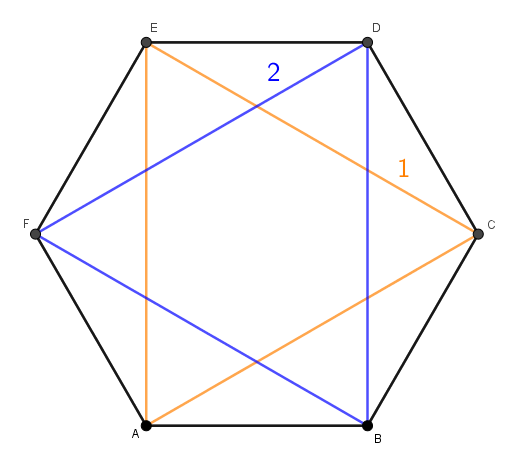
\includegraphics[scale=0.5]{haromszog.PNG}  \]
	
	Adott tehát $\varphi\colon D_6\to S_2$ hatás. Mi lesz a mag? Ami helyben hagyja mindkét háromszöget, másképpen mondva ami a sárga háromszöget helyben hagyja (hiszen ekkor a kék is automatikusan marad). Például benne van a magban az identitás, $f^2$, vagy $f^4$ is ahol $f$ a $60\degree$-os forgatás. De helyben hagyja őket az $FB$ szakaszfelező merőlegesére való $t$ tengelyes tükrözés is és ekkor persze $f^2\cdot t$ és $f^4\cdot t$ is. Összefoglalva:
	\[ \mathtt{Ker}\varphi = \{ id., f^2, f^4, t, f^2\cdot t, f^4\cdot t  \}  \]
	Másképpen mondva a sárga háromszöget a sárga háromszög szimmetriái hagyják helyben, ezek éppen $D_3$ elemei, vagyis $\mathtt{Ker}\varphi \cong D_3$.
	
	Mivel a képtér $S_2$, így a homomorfizmus-tétel alapján azt kaptuk, hogy $D_6/D_3 \cong S_2$.
	
	Nézzük most a főátlók esetét!
	
	\[ 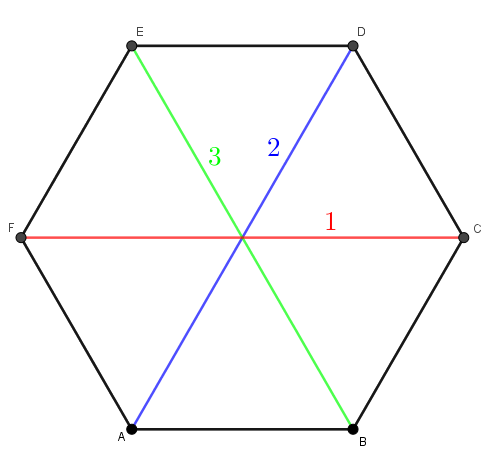
\includegraphics[scale=0.5]{atlo.PNG}  \]
	
	Itt most $\varphi\colon D_6 \to S_3$. Ebben az esetben azt látjuk, hogy ami helyben hagyja mindhárom átlót az csupán $2$ szimmetria: $id$ és $f^3$. Vagyis a mag: $\mathtt{Ker}\varphi = \{id, f^3\} \cong \Z_2$.
	
	Belátható, hogy $S_3$ minden eleme a képtérnek is eleme, például a
	$\begin{pmatrix}
		2 & 3
	\end{pmatrix}$
	benne van, hiszen az $FC$ egyenesére tükrözés képe éppen ez. Hasonlóan látható, hogy az összes többi transzpozíció is benne van, mivel pedig bármely elem előáll transzpozíciók szorzataként, így a teljes $S_3$ lesz a kép.
	
	Most tehát a homomorfizmus-tétel szerint $D_6/\Z_2 \cong S_3$.

	Könnyen belátható, hogy bármely $G$ csoportnak van legalább $2$ normálosztója, hiszen $\{1\} \triangleleft G$ és $G \triangleleft G$. Ezeket szokás \textbf{triviális normálosztó}knak nevezni.
	
	\begin{defi}
		Egy $G$ csoport \textbf{egyszerű}, ha a két triviális normálosztóján kívül más normálosztója nincs.
	\end{defi}

	Algebra és számelmélet 3 tárgyból láttuk korábban, hogy egyszerű csoport $A_5$.

	\begin{theo}[Feit-Thompson-tétel]
		Ha van egy páratlan elemű egyszerű csoportunk, az csak a $\Z_p$ lehet, vagyis $G$ egyszerű csoport esetén $2\nmid |G| \Rightarrow \exists p$ prím, melyre $G\cong \Z_p$.
	\end{theo}
	
	%, és egyszerű (véges $K$ test esetén) $PSL_n(K)$ is.
	
	%Hogy mi az a $PSL_n(K)$ azt leginkább úgy lehetne eddigi tanulmányainkhoz kötni, hogy algebra3-ból volt szó a $GL_n(K)$-ról, mely a $K$ test feletti $n\times n$-es invertálható mátrixok csoportja volt: general linear. Az invertálható mátrixok azzal a tulajdonsággal rendelkeznek, hogy determinánsuk $0$, egy speciális részcsoport az $SL_n(K)$, vagyis a speciális lineáris csoport, mely olyan $K$ test feletti $n\times n$-es mátrixokból áll, melyek determinánsa $1$. A $PSL_n(K)$ pedig a projektív speciális lineáris csoport, vagyis a projektív tér lineáris transzformációit leíró leképezésekhez tartozó $1$ determinánsú mátrixoké.
	
	\section{Direkt szorzat}
	
	A direkt szorzatról is már tanultunk algebra3-ból, így ez a fejezet is lényegében ismétlés csupán.
	
	\begin{defi}
		Az $A$ és $B$ halmazok direkt szorzata az $A$ és $B$ elemeiből képzett rendezett párok halmaza: $A\times B = \{ (a,b) \mid a\in A,\ b\in B \}$
	\end{defi}

	Azt is beláttuk korábban, hogy amennyiben $A$ és $B$ csoportok és definiálunk $A\times B$ elemein egy szorzást a következőképpen: $(a,b) \cdot (c,d) = (a\cdot c, b\cdot d)$, akkor az $A\times B$ halmaz csoportot alkot erre a szorzásra.
	
	Ennek bizonyítását most nem írom le újra, de a hozzá kapcsoló, előadáson ismét elhangzó tételeket igen, illetve emlék gyanánt az inverzképzés szabályát: $(a,b)^{-1} = (a^{-1}, b^{-1})$.
	
	\begin{lem}\label{dirlem1}
		Legyen $G$ csoport, melyben $A,B\triangleleft G$ normálosztók. Amennyiben a halmazok komplexusszorzata $A\cdot B = G$, akkor
		\begin{enumerate}
			\item{$A\cap B = \{1\}$}
			\item{$G$ csoport minden eleme egyértelműen áll elő egy $A$ és egy $B$ beli elem szorzataként}
		\end{enumerate}
		állítások ekvivalensek.
	\end{lem}

	\begin{proof} Külön-külön látjuk be a két irányt.
		
		\textit{1. $\Rightarrow$ 2. bizonyítása:}
		
		Annak jelentése, hogy $A\cdot B = G$ nem más, mint hogy $\forall g\in G$ esetén $\exists$ olyan $a\in A$ és $b\in B$, melyekre $a\cdot b=g$. Azt kell belátni, hogy $a$ és $b$ egyértelmű is!
		
		Tegyük fel, hogy létezik $a_1,a_2\in A$ és $b_1,b_2\in B$ melyek mindketten előállítják $g$-t, vagyis
		\[ a_1\cdot b_1 = g = a_2 \cdot b_2  \]
		balról $a_1^{-1}$-zel, jobbról $b_2^{-1}$-zel szorozva:
		\[ b_1\cdot b_2^{-1} = a_1^{-1} \cdot a_2 \]
		Viszont itt $b_1\cdot b_2^{-1} \in B$ és $a_1^{-1} \cdot a_2\in A$, ami azt jelenti, hogy mivel ez a két elem egymással egyenlő, ezért mindkét halmaznak eleme, tehát a metszetnek is. De a metszet egyetlen eleme az $1$, amiből következően:
		\[ b_1\cdot b_2^{-1} = 1 = a_1^{-1}\cdot a_2 \]
		ahonnan látszik, hogy $a_1=a_2$ és $b_1=b_2$, tehát tényleg egyértelmű az előállítás.
		
		\textit{2. $\Rightarrow$ 1. bizonyítása:}
		
		Indirekt tegyük fel, hogy $A$ és $B$ halmazoknak van más közös eleme is az $1$-en kívül, legyen ez $g\neq 1$. Ekkor azt állítom, hogy ellentmondást kapunk, mert $g$ kétféleképpen is előállítható, mégpedig:
		\[ g = g\cdot 1 = 1 \cdot g  \]
		ami azt jelenti, hogy az $a_1=g, b_1=1$ és $a_2=1, b_2=g$ különböző előállításai $g$-nek, hiszen $a_1\neq a_2$ és $b_1\neq b_2$.
	\end{proof}

	\begin{lem}\label{dirlem2}
		Legyen $G$ csoport, melyben $A,B\triangleleft G$ normálosztók. Ha $A\cap B = \{1\}$, akkor $\forall a\in A,\ b\in B$-re $a\cdot b = b\cdot a$.
	\end{lem}

	\begin{proof}
		Tekintsük a következő szorzatot:
		\[ b^{-1} \cdot a\cdot b \cdot a^{-1}  \]
		Na most ha $a\in A$ és $b\in B \Rightarrow b\in G$, akkor mivel $A$ normálosztó $G$-ben, ezért  rajta kívüli, $G$-beli elemekkel is zárt a konjugálásra, ami azt jelenti, hogy $b^{-1}\cdot a \cdot b\in A$, továbbá zárt inverzképzésre, tehát $a^{-1}\in A$, vagyis akkor ez az egész szorzat $A$-nak eleme. Akkor ennek a szorzatnak az inverze is eleme $A$-nak:
		\[ (b^{-1} \cdot a\cdot b \cdot a^{-1})^{-1} = a \cdot \color{red}b^{-1}\color{black} \cdot a^{-1} \cdot b \]
		Tekintsünk most erre $B$ szempontjából. Ott van egy $\color{red}b^{-1}\color{black}\in B$ elem megkonjugálva $a^{-1}\in A$ elemmel: $(a^{-1})^{-1} \cdot b^{-1} \cdot a^{-1} $, ez eleme $B$-nek, továbbá $b$ is. Tehát ez a valami $B$-nek is eleme és láttuk, hogy $A$-nak is.
		
		Mivel pedig $A\cap B = \{1\}$, ez csakis akkor lehetséges, ha ez maga az egységelem, akkor viszont a bal oldali valami is az egységelem volt, aminek az inverzét vettük (hiszen csak az egységelem inverze lehet az egységelem):
		\[ b^{-1}\cdot a \cdot b \cdot a^{-1} = 1 \]
		ahonnan balról szorozva $b$-vel, jobbról $a$-val adódik, hogy
		\[ a \cdot b = b\cdot a \]
		Éppen ezt akartuk.
	\end{proof}

	\begin{theo}
		Legyen $G$ csoport az $A$ és $B$ csoportok direkt szorzata: $G=A\times B$, tekintsük $A'=\{(a,1) \mid a\in A, 1\in B \}$ és $B'=\{(1,b) \mid 1\in A, b\in B  \}$ halmazokat. Ekkor
		\begin{enumerate}
			\item{$A',B' \triangleleft G$}
			\item{$A'\cap B' = \{(1,1)\}$}
			\item{$A' \cdot B' = G$}
		\end{enumerate}
		állítások teljesülnek.
	\end{theo}

	\begin{proof}
		Csak $A' \triangleleft G$ állítást látom be, $B'$-re hasonlóan megy. Az nyilvánvaló, hogy $A'\leq G$, hiszen
		\begin{itemize}
			\item{részhalmaza, mert az összes $(a,b)$ pár közül csak azokat tartalmazza, ahol $b=1$}
			\item{egységelem benne van $a=1$ választással}
			\item{zárt a szorzásra: $(a_1,1)\cdot (a_2,1)=(a_1\cdot a_2,1)\in A'$, mert $a_1\cdot a_2 \in A$}
			\item{zárt az inverzképzésre: $(a,1)^{-1}=(a^{-1},1)\in A'$, mert $a^{-1}\in A$}
		\end{itemize}
		Tehát azt kell még belátni, hogy zárt a konjugálásra $G$-ben, kell: $\forall a'\in A'$ és $g\in G$ esetén $g^{-1} \cdot a' \cdot g \in A'$. Legyen $a'=(a,1)$ és $g=(x,y)$, ekkor
		\[ g^{-1} \cdot a' \cdot g = (x^{-1},y^{-1})\cdot (a,1)\cdot (x,y) = (x^{-1}\cdot a \cdot x, y^{-1}\cdot 1 \cdot y) = (x^{-1}\cdot a\cdot x,1)\in A' \] 
		mert $x^{-1}\cdot a\cdot x \in A$.
		
		\textit{2. biz: }Ez nyilvánvaló, amennyiben $(x,y)$ elem benne van mindkét halmazban, akkor mindkét koordinátája $1$ kell legyen.
		
		\textit{3. biz: }
		Ez sem bonyolult, mivel $A'$ és $B'$ részcsoport $G$-ben, ezért elemeik szorzata nyilván nem vezethet kívül $G$-n, azt kell csak megmutatni, hogy minden $G$-beli elem előáll egy $A'$-beli és egy $B'$-beli szorzataként. Ha az ellenség ad egy $G$ beli $(x,y)$ elemet, akkor mi azt mondjuk neki, hogy $(x,1)\in A'$ és $(1,y)\in B'$ és
		\[ (x,1)\cdot (1,y) = (x\cdot 1,1\cdot y) = (x,y) \]
		tehát minden elem előáll szorzatként.
	\end{proof}

	\begin{theo}
		Legyen $G$ csoport, melyben van olyan $A$ és $B$ részcsoport, melyekre
		\begin{enumerate}
			\item{$A,B\triangleleft G$}
			\item{$A\cap B= \{1\}$}
			\item{$A\cdot B = G$}
		\end{enumerate}
		ekkor $G\cong A\times B$.
	\end{theo}

	\begin{proof}
		Izomorfizmus igazolásához meg kell adjunk egy bijektív leképezést a bal és jobb oldal között és igazoljuk, hogy szorzattartó. Legyen $(a,b)\in A\times B$, ekkor $\varphi\big((a,b)\big) =a\cdot b$ azt állítom, hogy jó leképezés lesz.
		
		Bijektív, mert minden $a\cdot b$ előáll képként (szürjektív) és a 2. tulajdonság és a \ref{dirlem1}. lemmánk miatt, minden $x\in G$ egyértelműen áll elő $(a,b)$ képe, vagyis $a\cdot b$ alakban (injektív).
		
		Szorzattartás igazolása: Kell, hogy ha $(a,b)\in A\times B$ és $(c,d)\in A\times B$, akkor szorzat képe a képek szorzata, vagyis
		\[ \varphi\big((a,b)\cdot (c,d)\big) = \varphi\big((a,b)\big) \cdot \varphi\big((c,d)\big)  \]
		bal oldalon elvégezve belül a szorzást
		\[ \varphi\big((ac,bd)\big) =\varphi\big((a,b)\big) \cdot \varphi\big((c,d)\big)  \]
		$\varphi$ általunk adott definíciója
		\[ (ac)\cdot (bd) = (ab)\cdot (cd) \]
		Csoportelemekről beszélünk, elhagyhatók a zárójelek és balról $a^{-1}$-zel, jobbról $d^{-1}$-zel szorozva egyszerűsödik a kifejezés
		\[ c\cdot b = b \cdot c  \]
		kellene teljesüljön és mivel végig ekvivalens átalakításokat csináltunk, ezért akkor a szorzattartás igaz volna. De hát ez teljesül is a tétel feltételei között megint csak a 2-es pont és a korábbi \ref{dirlem2}. lemmánk miatt $A$ és $B$ elemei között kommutatív a szorzás, kész vagyunk.
	\end{proof}

	Vegyük észre, hogy a bijekció miatt $G$ és $A\times B$ csoportnak ugyanannyi eleme van, sőt meg is feleltethetőek egymásnak. Azért kellett mégis izomorfizmust írnunk, mert a két csoport struktúrája hasonló, de nem ugyanaz! Az $A\times B$-ben $G$ elemeiből képezett rendezett párok vannak. Ugyanakkor az egyértelmű megfeleltetés miatt definiálhattuk volna $A\times B$-t úgy is, hogy az is $G$ elemeiből álljon. Éppen ezért a továbbiakban nem teszünk különbséget aközött, hogy $G\cong A\times B$ vagy $G = A\times B$.
	
	\begin{pl}
		Mutassuk meg, hogy $\Z_6=\Z_2\times \Z_3$.
		
		\begin{enumerate}
			\item Mivel Ábel-csoport esetén bármely részcsoport normálosztó, így $\Z_6 = \{0,1,2,3,4,5\}$ csoport normálosztója $\Z_2=\{0,3\}$ és $\Z_3=\{0, 2, 4\}$.
			
			\item Teljesül, hogy közös elemük csak az egységelem, tehát $\Z_2\cap \Z_3 = \{0\}$.
			
			\item Sőt az is igaz, hogy szorzatuk $\Z_2 \cdot \Z_3 = \Z_6$, hiszen $\Z_2$ másik (a $3$-as) eleme $\Z_3$-nak nem eleme, így $6$ féle különböző szorzat képezhető elemeikből, vagyis $\Z_6$ minden eleme előállítható.
		\end{enumerate}
	
		Az előző tétel szerint ekkor $\Z_6 = \Z_2 \times \Z_3$.
	\end{pl}
	
	\begin{pl}
		Lássuk be, hogy $D_6 = \Z_2 \times D_3$.
		
		Foglalkoztunk korábban a hatszög szimmetriáinak csoportjával és azt láttuk, hogy a háromszögek esetében is hatást kapunk, melynek magja $\mathtt{Ker}\varphi \cong D_3$-mal, illetve átlók esetében $\mathtt{Ker}\varphi \cong \Z_2$.
		\begin{enumerate}
			\item Mivel a mag mindig normálosztó, így $\Z_2 \triangleleft D_6$ és $D_3\triangleleft D_6$.
			
			\item Teljesül, hogy közös elemük csupán az identitás, tehát $D_3\cap \Z_2 = \{id.\}$.
			
			\item Sőt az is igaz, hogy szorzatuk $\Z_2 \cdot D_3 = D_6$, hiszen $\Z_2$ másik (vagyis $f^3$) eleme $D_3$-nak nem eleme, így $12$ féle különböző szorzat képezhető elemeikből, vagyis $D_6$ minden eleme előállítható.
		\end{enumerate}
		Az előző tétel szerint ekkor $D_6 = \Z_2 \times D_3$.
	\end{pl}
	Tanultuk tavaly, hogy a kocka szimmetriái (amiből 48 van) hat a testátlók és a beírt tetraéderek halmazán is.
	\[ 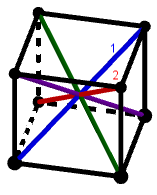
\includegraphics[scale=1]{kocka_testatlo.png} \hspace{72pt} 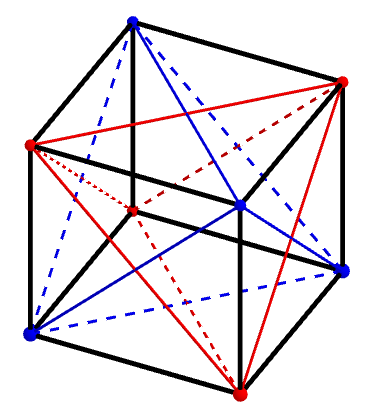
\includegraphics[scale=0.5]{kocka_tetraederek.png}  \]
	%kép a teljes S_4, tehát 24 elemű, orbit-stab lemma
	A testátlók esetében belátható, hogy a magban csupán $2$ transzformáció lesz: a helybenhagyás és a középpontos tükrözés: $\mathtt{Ker}\varphi = \{id., k\}\cong \Z_2$.
	
	Tetraéderek esetében pedig az lesz a mag, ami az egyik tetraédert helyben hagyja (hiszen akkor a másik is helyben marad), vagyis a tetraéder szimmetriáinak csoportja: $S_4$.
	
	\begin{pl}
		Bizonyítsuk be, hogy a kocka szimmetriáinak $K$ csoportjára $K = \Z_2 \times S_4$.
		
		\begin{enumerate}
			\item Mivel a mag mindig normálosztó, így $\Z_2 \triangleleft K$ és $S_4\triangleleft K$.
			
			\item Teljesül, hogy közös elemük csupán az identitás (hiszen a középpontos tükrözés pont megcseréli a tetraédereket), tehát $\Z_2 \cap S_4 = \{id.\}$.
			
			\item Sőt az is igaz, hogy szorzatuk $\Z_2 \cdot S_4 = K$, hiszen $\Z_2$ másik (vagyis $k$) eleme $S_4$-nek nem eleme, így $48$ féle különböző szorzat képezhető elemeikből, vagyis $K$ minden eleme előállítható.
		\end{enumerate}
		
		Most is teljesül a három feltétel, tehát $K = \Z_2 \times S_4$.
	\end{pl}
	
	\begin{theo}[Ábel-csoportok alaptétele]
		Ha $A$ Ábel-csoport, akkor $A$ előáll a következő alakban:
		\[ A = \Z_{p_1}^{\alpha_1} \times \Z_{p_2}^{\alpha_2} \times \ldots \times \Z_{p_k}^{\alpha_k} \]
		ahol $\forall p_i$ prím és a felbontás a prímhatványok erejéig egyértelmű (tehát maga a felbontás nem egyértelmű, de a prímhatványok igen).
	\end{theo}
	
	Például $\Z_6 = \Z_3 \times \Z_2$, hiszen $6 = 2^1\cdot 3^1$. Hasonlóan mondhatjuk, hogy mivel $18 = 2^1\cdot 3^2$, így $\Z_{18} = \Z_2 \times \Z_9$.
	
	%Ugyanakkor %az Ábel-csoportok alaptétele nem szól arról, hogy az egyes prímeknek különböznie kell, így 
	%könnyen láthatóan $\Z_{18} = \Z_2 \times \Z_3 \times \Z_3$ egy másik felbontást ad, amely előbbivel sem izomorf, mert ebben a maximális elemrend $3$, míg $\Z_2 \times \Z_9$ esetén van $9$ rendű elem is. Ebből láthatjuk, hogy a prímhatványok is csak akkor egyértelműek, hogy ha minden $p_i$ különböző.
	
	\chapter{Csoportelmélet}
	\section{Centralizátor és centrum}
	
	Tanultunk korábban a konjugálás műveletéről, jelölésben használtuk $h$-nak a $g$-vel vett konjugáltjára a $g^{-1}\cdot h\cdot g$ jelölést és a $h^g$ jelölést is. Utóbbi a hatványozás művelete miatt megtévesztő lehet, így amennyiben lehetséges én a továbbiakban mellőzöm a használatát.
	
	Volt szó arról, hogy a konjugálás ekvivalencia reláció, így osztályokra bontja a $G$ csoportot, ezeket neveztük \textbf{konjugáltosztály}oknak:
	\[ \mathcal{K}(a) = \{b \in G \mid \exists x\in G\colon x^{-1} \cdot g \cdot x = b  \}  \]
	vagyis egy $g$ elem konjugáltosztályán azon elemek halmazát értjük, melyekbe "átkonjugálódhat", vagy másképp fogalmazva eljuthat konjugálás által.
	
	\begin{defi}
		Egy $a\in G$ csoportelem \textbf{centralizátor}án azon csoportbeli elemek halmazát értjük, melyekkel $a$ felcserélhető a csoporton definiált szorzás műveletére:
		\[ C_G(a) = \{ h\in G \mid a\cdot h = h\cdot a  \}  \]
	\end{defi}

	\begin{theo}
		Egy $a\in G$ elem centralizátora mindig részcsoportot alkot $G$-ben: $C_G(a) \leq G$.
	\end{theo}

	\begin{proof}
		Részcsoport teszt: zártság szorzásra, inverzképzésre, egységelemet tartalmazza-e:
		\begin{itemize}
			\item Nyilván $1\in C_G(a)$ hiszen $1\cdot a = a\cdot 1$ teljesül $\forall a\in G$ esetén.
			\item Szorzásra zártság: $g,h\in C_G(a)$, vagyis $ga = ag$ és $ha=ah$, kellene $g\cdot h = \in C_G(a)$, vagyis $gh\cdot a = a\cdot gh$ ami nyilván teljesül, hiszen egyesével elvégezve a cseréket $gh\cdot a = g\cdot a \cdot h = a \cdot gh$
			\item Inverzképzésre zártság: $g\in C_G(a)$, vagyis $ga=ag$ esetén természetesen mindkét oldalról $g^{-1}$-zel szorozva kapjuk, hogy $a\cdot g^{-1} = g^{-1} \cdot a$, ami éppen azt jelenti, hogy $g^{-1}\in C_G(a)$.
		\end{itemize}
	\end{proof}
	
	Észrevétel: a centralizátor elemei éppen azok, amelyek átkonjugálják az $a$ elemet önmagába, hiszen ha $ah = ha$ akkor $h^{-1}\cdot a \cdot h = a$ teljesül.
	
	\begin{theo}\label{konjcentr}
		Az $a\in G$ elem esetén $|\mathcal{K}(a)| \cdot |C_G(a)| = |G|$.
	\end{theo}

	\begin{proof}
		Ha már $C_G(a)\leq G$, akkor beszélhetünk a centralizátor jobboldali mellékosztályairól. Könnyen belátható, hogy az egyes jobboldali mellékosztályok elemeinek van egy közös tulajdonsága: mindannyian ugyanoda konjugálják az $a$ elemet. Vagyis $x\in C_G(a)\cdot y$ esetén $x$ és $y$-nal képzett konjugáltja $a$-nak megegyezik.
		
		Ez könnyen látható, hiszen $x\in C_G(a)\cdot y$ esetén $x\cdot y^{-1} \in C_G(a)$, vagyis $x\cdot y^{-1}$ elemmel felcserélhető az $a$ elem, azaz:
		\[ x\cdot y^{-1} \cdot a = a \cdot x \cdot y^{-1}  \]
		balról $x^{-1}$-el, jobbról $y$-al szorozva $x^{-1}\cdot a \cdot x = y^{-1} \cdot a \cdot y$ adódik, vagyis éppen azt kapjuk, hogy $a$-nak az $x$ és $y$ szerinti konjugáltja megegyezik.
		
		Ezek alapján a $G$ csoportnak a $C_G(a)$ részcsoport szerint éppen annyi mellékosztálya van, ahány konjugáltja $a$ elemnek, vagyis a mellékosztályok száma $a$ konjugáltosztályának elemszáma: $|\mathcal{K}(a)|$. 
		
		Lagrange-tétele alapján a csoport elemszáma megegyezik egy részcsoport elemszámának és azon részcsoport szerinti mellékosztályok számának szorzatával, így: $|\mathcal{K}|\cdot |C_G(a)| = |G|$.
	\end{proof}

	Ezen utóbbi tétel egy másik megfogalmazása a következő.
	
	\begin{theo}
		Egy $G$ csoport hat önmagán konjugálással, vagyis $\varphi\colon G\to S_G$ leképezés, melyre $\varphi(g) = \pi\in S_G$, melyre $\pi(h) = g^{-1}\cdot h \cdot g$ permutáció egy homomorfizmus.
	\end{theo}

	\begin{proof}
		Van most egy furcsa $\varphi$ leképezésünk, mely minden csoportbeli elemhez egy olyan permutációt rendel, mely esetén minden csoportbeli elem képe a $g$-vel vett konjugáltja. Tehát most $\varphi$ egy $g$ elemhez hatás lévén egy függvényt rendel! Azt kell belátnunk, hogy művelettartóan teszi mindezt.
		
		\begin{itemize}
			\item Szorzástartó: Kellene, hogy $g_1$ és $g_2$ elemek esetén $\varphi(g_1\cdot g_2) = \varphi(g_1) \cdot \varphi(g_2)$. Mit rendel $g_1$-hez $\varphi$? Egy olyan permutációt, amely minden $h$ elemhez a konjugáltját rendeli. Hasonlóan $g_2$ esetében:
			\[ \varphi(g_1) = h \to g_1^{-1}\cdot h \cdot g_1 \hspace{10mm} \text{és} \hspace{10mm} \varphi(g_2) = h \to g_2^{-1} \cdot \color{red} h \color{black} \cdot g_2  \]
			Mi lesz ekkor $\varphi(g_1)\cdot \varphi(g_2)$? Egyszerűen az elemekhez rendelt permutációkat is össze kell "szoroznunk", ami permutációk esetén természetesen kompozíciót jelent: az első $h$-t elviszi $g_1^{-1}\cdot h\cdot g_1$-be, majd a második ezt az elemet konjugálja tovább:
			\[ \varphi(g_1)\cdot \varphi(g_2) = h\to g_1^{-1} \cdot h \cdot g_1 \to g_2^{-1} \cdot \color{red} g_1^{-1} \cdot h \cdot g_1 \color{black} \cdot g_2 = h \to g_2^{-1} \cdot g_1^{-1} \cdot h \cdot g_1 \cdot g_2 \]
			átírva az inverzet:
			\[ = (g_1\cdot g_2)^{-1} \cdot h \cdot g_1 \cdot g_2 = \varphi(g_1\cdot g_2)  \]
			\item Inverztartó: Kellene, hogy $\varphi(g)^{-1} = \varphi(g^{-1})$:
			\[ \varphi(g)^{-1} = (h\to g^{-1} \cdot h \cdot g)^{-1} = g^{-1} \cdot h \cdot g \to h = h \to g\cdot h \cdot g^{-1}  = \varphi(g^{-1}) \]
		\end{itemize}
		Egy $a$ elem pályáján azon $G$-beli elemeket értettük, ahová $\varphi$ hatás által eljuthat $a$. Vagyis a $g^{-1} \cdot a \cdot g$ elemek halmazát, így ebben az esetben az orbit éppen az $a$ elem konjugáltosztálya lesz: $\mathcal{K}(a)$.
		
		Másik fontos észrevétel, hogy, mely elemek hagyják fixen $a$-t? Vagyis melyek azon $g\in G$ elemek, melyekkel képzett konjugáltja önmaga? Ezek éppen a centralizátor elemei, tehát jelenlegi $\varphi$ csoporthatás esetén egy $a\in G$ elem stabilizátora éppen a centralizátora: $C_G(a)$.
		
		És az orbit-stabilizátor lemma szerint ismét megkaptuk az előző tétel állítását, vagyis, hogy $|\mathcal{K}(a)| \cdot |C_G(a)| = |G|$.
	\end{proof}
	
	\textbf{Emlék:} Egy $
	\begin{pmatrix}
	1 & 2 & \ldots & n\\
	\end{pmatrix}$ ciklus konjugáltja egy $\sigma$ permutációval: 
	\[  \sigma^{-1} \cdot 
	\begin{pmatrix}
	1 & 2 & \ldots & n\\
	\end{pmatrix}
	\cdot \sigma = 
	\begin{pmatrix}
	\sigma(1) & \sigma(2) & \ldots & \sigma(n)\\
	\end{pmatrix} \]
	
	\begin{pl}
		Határozzuk meg $S_4$-ben $\pi = \begin{pmatrix}
		1 & 2 & 3 & 4 \\
		\end{pmatrix}$ permutáció centralizátorát!
		
		Tudjuk, hogy a centralizátor azon $\sigma$ permutációk halmaza, melyekkel felcserélhető, vagyis
		\[ \begin{pmatrix}
		1 & 2 & 3 & 4 \\
		\end{pmatrix} \cdot \sigma = 
		\sigma \cdot
		\begin{pmatrix}
		1 & 2 & 3 & 4 \\
		\end{pmatrix}  \]
		vagyis azon $\sigma$ permutáció, mely önmagába konjugálja:
		\[ \sigma^{-1} \cdot 
		\begin{pmatrix}
		1 & 2 & 3 & 4 \\
		\end{pmatrix}
		\cdot \sigma = 
		\begin{pmatrix}
		1 & 2 & 3 & 4 \\
		\end{pmatrix} =
		\begin{pmatrix}
		\sigma(1) & \sigma(2) & \sigma(3) & \sigma(4) \\
		\end{pmatrix} \]
		Ha $\begin{pmatrix}
		1 & 2 & 3 & 4 \\
		\end{pmatrix}$ permutáció konjugáltja is ugyanezen ciklus kell legyen, akkor $\sigma$ négyféleképpen választható meg:
		\begin{small}
		\[ \sigma = 
		id. \hspace{5mm} \text{vagy} \hspace{5mm} \sigma = 
		\begin{pmatrix}
		1 & 2 & 3 & 4 \\
		2 & 3 & 4 & 1 \\
		\end{pmatrix} \hspace{5mm} \text{vagy} \hspace{5mm} \sigma = 
		\begin{pmatrix}
		1 & 2 & 3 & 4 \\
		3 & 4 & 1 & 2 \\
		\end{pmatrix}
		\hspace{5mm} \text{vagy} \hspace{5mm} \sigma = 
		\begin{pmatrix}
		1 & 2 & 3 & 4 \\
		4 & 1 & 2 & 3 \\
		\end{pmatrix} \]
		\end{small}
	    így tehát a $\sigma = 
		\begin{pmatrix}
		1 & 2 & 3 & 4 \\
		\end{pmatrix}$ permutáció centralizátora négy elemű, elemei a lehetséges $\sigma$ permutációk, avagy $
		\begin{pmatrix}
		1 & 2 & 3 & 4 \\
		\end{pmatrix}$ hatványai, hiszen egy ciklus a saját hatványaival mindig felcserélhető.
		
		Másképpen is megállapíthattuk volna ezt, például ha centralizátora helyett konjugáltosztályát vizsgáljuk. Tudjuk, hogy egy permutáció konjugáltja azonos ciklus szerkezetű, ezért
		$\begin{pmatrix}
		1 & 2 & 3 & 4 \\
		\end{pmatrix}$ konjugáltosztályában $4$ hosszú ciklusok szerepelnek. Hány darab van belőlük? Hányféleképpen lehet $4$ elemet ciklikusan permutálni? Rögzítjük az első helyét, majd a második helyre $3$ féle elem kerülhet, a harmadik helyre $2$ féle, majd végül az utolsóra $1$ féle, így $3\cdot 2 \cdot 1= 6$ elemű a konjugáltosztálya. Mivel $|S_4| = 24$, így a \ref{konjcentr}. tétel alapján
		\[ \left|C_G\left(\begin{pmatrix}
		1 & 2 & 3 & 4 \\
		\end{pmatrix}\right)\right| = \dfrac{|S_4|}{\left|\mathcal{K}\left(\begin{pmatrix}
			1 & 2 & 3 & 4 \\
			\end{pmatrix}\right)\right|} = \dfrac{24}{6} = 4  \]
		ahonnan ismét látjuk, hogy $\begin{pmatrix}
		1 & 2 & 3 & 4 \\
		\end{pmatrix}$ centralizátorában $4$ elem van csupán, és mivel saját hatványaival mindig felcserélhető, így centralizátora a hatványaiból álló (generált ciklikus) részcsoport $C_{S_4} \left(\begin{pmatrix}
		1 & 2 & 3 & 4 \\
		\end{pmatrix}\right) = \left \langle \begin{pmatrix}
		1 & 2 & 3 & 4 \\
		\end{pmatrix} \right \rangle $.
	\end{pl}

	Mit kapok ha veszem minden $a\in G$ elem centralizátorának a metszetét? Olyan elemeket, amelyek $G$ bármely elemével felcserélhetőek, ezek halmazát szokás centrumnak nevezni.
	
	\begin{defi}
		Egy $G$ csoport \textbf{centrum}a alatt a $Z(G) = \{ g\in G \mid \forall h\in G\colon gh = hg  \}$ halmazt értjük.
	\end{defi}

	\begin{theo}\label{centnorm}
		Csoport centruma normálosztója a csoportnak: $Z(G)\triangleleft G$.
	\end{theo}

	\begin{proof}
		Be kell látnunk, hogy részcsoport és zárt a konjugálásra.
		
		\begin{itemize}
			\item Szorzásra zárt: $g_1, g_2 \in Z(G)$ esetén $\forall h\in G$-re $g_1\cdot h = h \cdot g_1$ és $g_2 \cdot h = h \cdot g_2$ teljesül, így
			\[ g_1 \cdot g_2 \cdot h = g_1 \cdot h \cdot g_2 = h \cdot g_1 \cdot g_2  \]
			miatt $g_1\cdot g_2 \in Z(G)$
			\item Egységelem benne van nyilván: $1\in Z(G)$
			\item Inverzképzésre zárt: $g\in Z(G)$ esetén $\forall h\in G$-re $gh=hg$, vagyis mindkét oldalról $g^{-1}$-zel szorozva $h\cdot g^{-1} = g^{-1} \cdot h$, így $g^{-1} \in Z(G)$.
			\item Konjugálásra zárt: $g\in Z(G)$ esetén $x^{-1} \cdot g \cdot x \in Z(G)$, hiszen ha $g\in Z(G)$ akkor $gx=xg$, vagyis $x^{-1}\cdot g \cdot x = x^{-1} \cdot x \cdot g = g \in Z(G)$.
			Megjegyzés: Centrumbeli elemek konjugáltosztálya egyelemű, így mikor azt kérdezzük, hogy $g$ centrumbeli elem összes konjugáltja benne van-e $Z(G)$-ben, akkor nyilvánvalóan igen, hiszen egyetlen konjugáltja önmaga.
		\end{itemize}
	\end{proof}
	
	\begin{pl}
		Határozzuk meg $Z(S_4)$-et!
		
		A centrum elemei minden csoportbeli elemmel felcserélhetőek, így egy centrumbeli elem felcserélhető kell legyen konkrétan a $\begin{pmatrix}
		1 & 2 & 3 & 4 \\
		\end{pmatrix}$ ciklussal is, mellyel láttuk, hogy csak saját hatványai cserélhetők fel, így $Z(G) \subseteq \left \langle \begin{pmatrix}
		1 & 2 & 3 & 4 \\
		\end{pmatrix} \right \rangle$. Ugyanakkor hasonlóan elmondható ez $\begin{pmatrix}
		1 & 3 & 2 & 4 \\
		\end{pmatrix}$ ciklussal is, így az általa generált ciklikus csoportnak is részhalmaza a centrum. Igen ám, csakhogy ezen két darab $4$ elemű csoportoknak egyetlen közös eleme az identitás, így $Z(G) = \{id.\}$.
	\end{pl}

	\begin{mj}
		Az előző példa elmondható lett volna tetszőleges $S_n$ esetében, így a permutációcsoportok centruma nem túlságosan izgalmas: $Z(S_n) = \{id.\}$.
	\end{mj}

	\begin{pl}
		Határozzuk meg $D_4$ és $D_5$ centrumát!
		
		Lehet-e egy tükrözés a centrumban? Nem lehet, mivel egy tükrözés nem cserélhető fel minden elemmel, hiszen minden tükrözés esetén tudunk mondani legalább egy olyan másik tükrözést amellyel nem cserélhető fel, hiszen különböző sorrendben szorozva őket, különböző irányú forgatásokhoz jutunk.
		
		Így tehát a centrumban biztosan csak fogatások lehetnek. Azok közül is csak különlegesek, hiszen egy $f^n$ forgatás csakis akkor lehet a centrumban, amennyiben egy $t$ tengelyes tükrözéssel felcserélhető, vagyis:
		\[ t\cdot f^n = f^n \cdot t  \]
		ugyanakkor tudjuk, hogy $t\cdot f^n = f^{-n} \cdot t$, tehát azt a szükséges feltételt kaptuk\footnote{Ez egyben elégséges feltétel is, hiszen a forgatások felcserélhetők egymással.}, hogy:
		\[ f^n \cot t = f^{-n} \cdot t  \]
		amelyet $t$-vel egyszerűsítve $f^n = f^{-n}$ feltételhez jutunk, vagyis csakis olyan forgatás felelhet meg nekünk, amely önmaga inverze. Ilyet csak kettőt ismerünk, az identitást és a $180\degree$-os forgatást, vagyis $Z(D_4) = \{id., f^2\}$. %így $f^n$ szögét $\alpha$-val jelölve, az meg kell egyezzen modulo $2\pi$ az $f^{-n}$ forgatás szögével, amely $-\alpha$: $\alpha \equiv \alpha\ (2\pi)$ vagyis $2\cdot \alpha \equiv 0\ (2\pi)$, ahonnan $\alpha \equiv 0\ (\pi)$. Ennek csakis a $\pi$ és $2\pi$ szöggel való elforgatás tesz eleget, vagyis a 
		
		Az ötszög szimmetriái esetében annyit változik a problémánk, hogy középpontos tükrözés nincs a diédercsoportban, így $Z(D_5) = \{id.\}$.	\end{pl}
	
		\begin{mj}
			Hasonlóan meggondolva tetszőleges $D_n$ diédercsoport centruma: $Z(D_{2n+1}) = \{id.\} $, illetve $Z(D_{2n}) = \{id., f^n\}$.
		\end{mj}

	
	\section{Prímek és csoportok}
	
	Lagrange tétele szerint ha $H\leq G$, akkor $|H| \mid |G|$. Igaz-e a tétel megfordítása olyan értelemben, hogy ha egy szám osztja a csoport rendjét, akkor létezik olyan részcsoport, amelynek éppen az az elemszáma? Nem igaz, például belátható, hogy $|A_4|=\frac{4!}{2} = 12$ és $6\mid 12$, de nem létezik $A_4$-nek $6$ elemű részcsoportja.
	
	Hasonló kérdés merülhet fel elemrendek esetén, ugyanis tanultuk, hogy bármely elem rendje osztja a csoport rendjét: $a\in G$ esetén $o(a)\mid |G|$. Ugyanakkor az nem igaz, hogy ha $b\mid |G|$, akkor van olyan eleme $G$-nek, amelynek rendje éppen $b$. Például $D_6$ esetében $4\mid 12 = |D_6|$, de nem létezik olyan elem $D_6$-ban, amelynek rendje $4$, hiszen a tükrözések rendje $2$, a forgatásoké pedig $o(f) = 6$, $o(f^2) = 3$, $o(f^3) = 2$, $o(f^4) = 3$, és $o(f^5) = 6$. Ha viszont az osztó egy $p$ prímszám, akkor már létezik $p$ rendű elem.
	
	\begin{theo}[Cauchy]
		Ha $p\mid |G|$ akkor $\exists g\in G\colon o(g) = p$.
	\end{theo}

	\begin{proof}
		Képezzünk $G$ elemeiből rendezett $p$-eseket a következő módon: $(g_1,g_2,\ldots,g_p)$ legyen egy rendezett $p$-es, akkor ha
		\[ g_1 \cdot g_2 \cdot \ldots g_p = 1  \]
		Nyilvánvaló, hogy tudunk ilyen elem $p$-est képezni, például $\forall g_i = 1$ számunkra megfelelő.
		
		Az is könnyen meghatározható, hogy hány darab ilyet tudunk képezni: tetszőlegesen megválaszthatjuk $G$ elemei közül az első $p-1$ ilyen elemet, melyeket bárhogyan is választunk meg és $a = g_1 \cdot g_2 \cdot \ldots g_{p-1}$ szorzatukat tekintjük, az utolsó $g_p$ elem mindig egyértelműen megválasztható lesz $g_p = a^{-1}$. Éppen ezért annyi ilyen elem $p$-est tudunk készíteni, ahányféleképpen az első $p-1$ elem megválasztható, tehát: $|G|^{p-1}$.
		
		Hasznos észrevétel, hogy ha $(g_1,g_2,\ldots, g_p)$ egy számunkra megfelelő $p$-es volt, akkor jó lesz $(g_2,\ldots, g_p, g_1)$ is, hiszen balról $g_1^{-1}$-el, jobbról $g_1$-vel szorozva:
		\[ g_1\cdot g_2\cdot \ldots \cdot g_p = 1 \hspace{5mm} \Rightarrow \hspace{5mm} g_2 \cdot \ldots \cdot g_p \cdot g_1 = g_1^{-1} \cdot g_1 = 1  \]
		Ez azt jelenti, hogy egy megfelelő rendezett $p$-est találva egyben annak ciklikus elforgatottjai is jó rendezett $p$-esek. 
		
		Hányféle különböző elforgatottja lehet egy rendezett $p$-esnek? Azt állítom, hogy vagy $p$ vagy csak $1$. Amennyiben ugyanis van neki $2$ azonos elforgatottja, akkor könnyen belátható, hogy a rendezett $p$-es minden eleme megegyezik.
		
		Például ha $3$-al elforgatva egy rendezett $p$-est önmagát kapjuk, akkor
		\[ (\color{red} g_1 \color{black}, g_2, g_3, \color{blue} g_4 \color{black}, g_5, g_6, g_7, \ldots, g_p) = (\color{red} g_4 \color{black}, g_5, g_6, \color{blue} g_7 \color{black} \ldots, g_p, g_1, g_2, g_3)  \]
		$\color{red} g_1 \color{black} = \color{red} g_4 \color{black}$ illetve $\color{blue} g_4 \color{black} = \color{blue} g_7 \color{black}$ és így tovább. Vagyis ha $3$-al elforgatva önmagát kapom akkor minden elem megegyezik az őt követő harmadikkal.
		
		NODE! Akkor $a_1$ elemmel megegyezik bármely, tőle $3k$-ra lévő elem, vagyis az összes $3k+1$ indexű elem. Vagyis az $a_1$ elemmel azok az $a_b$ elemek egyeznek meg, melyek esetén tudunk mondani olyan $k$-t, hogy $3k+1 \equiv b\ (p)$. Könnyen látható, hogy ez bármely $b$ esetén teljesül, hiszen $3k\equiv b-1\ (p)$ kongruencia mindig megoldható $k$-ra, mivel $(3,p) = 1$.
		
		Ezzel tehát beláttuk, hogy egy rendezett $p$-es minden elforgatottja megegyezik, ha van két azonos eleme. Tehát innentől kezdve két esetet vizsgálunk, amikor a rendezett $p$-es minden eleme azonos, és amikor minden eleme különbözik.
		
		Vannak olyan $g$ elemek, amelyekből $p$ darabot véve kapunk egy jó rendezett $p$-est melynek minden eleme azonos. Ez éppen azt jelenti, hogy $g^p = 1$. Nem tudjuk hány ilyen elem van, de egy darab biztosan, az $1$. Továbbiakban jelölje $x$ azon $g$ elemek számát melyre teljesül $g^p=1$.
		
		Nézzük egy picit a másik esetet, amikor a rendezett $p$-es minden eleme különbözik. Hány darab ilyen van? Jelöljük ezt mondjuk $y$-al. Ha találunk egy $p$ különböző elemből egy rendezett $p$-est, akkor annak bármely elforgatottja is jó rendezett $p$-es számunkra, tehát ha találunk egy jó, csupa különböző elemből álló rendezett $p$-est, akkor azzal együtt igazából $p$ darabot találtunk egyszerre. Ez azt jelenti, hogy a különböző elemekből álló jó rendezett $p$-esek számát osztja $p$, vagyis: $p\mid y$.
		
		Összesen hány jó $p$-es létezik? Kiszámoltuk, hogy $|G|^{p-1}$. De úgy is mondhatnánk, hogy ahány jó csupa azonos, és ahány jó csupa különböző elemű, vagyis
		\[ |G|^{p-1} = x + y  \]
		Most használjuk ki a tétel feltételét, hogy $p\mid |G|$, ekkor persze $p\mid |G|^{p-1}$ is teljesül, illetve láttuk, hogy $p\mid y$, így adódik az előbbi egyenletből, hogy $p\mid x$.
		
		Viszont ez azt jelenti, hogy $p$ osztja azon $g$ elemek számát, melyeket $p$-edik hatványra emelve $1$-et kapunk. Viszont mivel $p\nmid 1$, így ezek száma több mint $1$, vagyis az $1$ elemen kívül most már látjuk, hogy ténylegesen létezik még olyan $g\neq 1$ elem, melyre $g^p=1$. Viszont ez azt is jelenti, hogy $o(g) = p$, hiszen $g$-re nézve a $p$ egy jó kitevő, márpedig a jó kitevőket osztja a rend, tehát $p$ osztójaként $o(g) = p$ vagy $o(g) = 1$ jöhet csak szóba, de utóbbi esetében $g = 1$ teljesülne, viszont mi olyan $g$-t is tudtunk választani, mely az egységelemtől különbözik.
	\end{proof}

	Egy csoport centrumának mindig eleme az egységelem, hiszen az minden elemmel felcserélhető. Amennyiben egy csoport centruma csupán az $1$ elemet tartalmazza, akkor a \textbf{triviális centrum} elnevezést szokás használni.
	
	\begin{theo}\label{prcentr}
		Prímhatványrendű csoport centruma nem triviális: $|G|=p^n \hspace{2mm} \Rightarrow \hspace{2mm} |Z(G)| > 1$.
	\end{theo}

	\begin{proof}
		Bontsuk fel a $G$ csoportot konjugáltosztályok uniójára\footnote{Ezt az egyenletet neveztük előadáson \textbf{osztályegyenlet}nek is.}:
		\[ G = \bigcup \mathcal{K}(a)  \]
		Láttuk a \ref{centnorm}. tételben, hogy a centrum is normálosztó, így $Z(G)$ is előáll konjugáltosztályok uniójaként. Válasszuk ebben az unióban két részre a halmazokat, vegyük azon a konjugáltosztályokat, melyek előállítják $Z(G)$-t, illetve azokat, melyek elemei nem centrumbeliek:
		\[ G = Z(G) \cup  \bigcup_{a\notin Z(G)} \mathcal{K}(a)  \]
		Ha ezek a halmazok megegyeznek, akkor számosságuk is, mivel pedig a jobboldali unióban szereplő halmazok diszjunktak, így uniójuk számossága a számosságaik összege:
		\[ |G| = |Z(G)| + \sum_{a \notin Z(G)} |\mathcal{K}(a)|  \]
		Mivel $|G|=p^n$, és \ref{konjcentr}. tétel miatt $|\mathcal{K}(a)|\cdot |C_G(a)| = |G|$ teljesül, így $|\mathcal{K}(a)|$ csakis $p^n$ osztója, vagyis prímhatvány lehet. Sőt még azt is tudjuk, hogy ha nem egy centrumbeli konjugáltosztályról van szó, akkor $|\mathcal{K}(a)|\neq 1$, hiszen ha $a$ elem konjugáltosztálya egyelemű lenne, akkor minden elemmel felcserélhető lenne $a$, vagyis centrumbeli elem lenne. Ezek szerint $p$-vel osztható az összes $|\mathcal{K}(a)|$.
		
		Viszont ekkor $p \bigm| |Z(G)|$ is teljesül, így $|Z(G)| > 1$.
	\end{proof}
	
	\begin{theo}\label{indexnorm}
		Ha egy $G$ csoport $H$ részcsoportjának indexe $2$, akkor $H$ normálosztó: $H\leq G$ és $|G:H|=2 \hspace{2mm} \Rightarrow \hspace{2mm} H\triangleleft G$.
	\end{theo}
	
	\begin{proof}
		Mivel $H$ indexe $2$, így $H$-nak két különböző (jobboldali) mellékosztálya van, vagyis $H\neq G$, így $\exists g\in G$, melyre $g\notin H$.
		
		Ekkor $H\neq H\cdot g$, hiszen utóbbi tartalmazza $g$ elemet, tehát mellékosztályokra bontva $G$ csoportot: $G=H\cup H\cdot g$, másképp fogalmazva $H\cdot g = G\setminus H$.
		
		Hasonlóan baloldali mellékosztállyal $H \neq g\cdot H$, hiszen utóbbi tartalmazza $g$ elemet, tehát mellékosztályokra bontva: $G=H\cup g\cdot H$, másképp $g\cdot H = G\setminus H$.
		
		Innen pedig azt kaptuk, hogy $H\cdot g = g \cdot H$, ami a normálosztó $g^{-1} \cdot H \cdot g = H$ tulajdonságnak egy ekvivalens átfogalmazása.
	\end{proof}

	\begin{mj}
		Másképp fogalmazva, ha találunk egy $H$ részcsoportot, melynek elemszáma éppen $|H| = \frac{|G|}{2}$, akkor azonnal adódik, hogy az normálosztó is.
	\end{mj}

	Érdekes észrevétel, hogy amennyiben $G$ csoport kommutatív, akkor minden elem mindennel felcserélhető, tehát minden elem a centrumban van, így $Z(G) = G$. Mivel $Z(G)$ normálosztó, így tekinthetem $G$-nek a $Z(G)$ szerinti faktorcsoportját, melynek elemszáma:
	\[ |G/Z(G)| = \dfrac{|G|}{|Z(G)|}  \]
	vagyis jelen esetben $1$, mégpedig egyetlen eleme $Z(G) = G$. Ekkor persze ez az egyelemű $\{G\}$ csoport ciklikus de ez nem túl izgalmas, mert az $1$ elemű csoportról sok érdekeset nem tudunk megállapítani. Tekintsük helyette azt, amikor $G$ nem kommutatív.

	\begin{theo}\label{zgNemCikl}
		Tetszőleges $G$ nemkommutatív csoport esetén $G/Z(G)$ nem ciklikus.
	\end{theo}
	
	\begin{proof}
		Indirekt tegyük fel, hogy $G$ nem kommutatív, de $G/Z(G)$ mégis ciklikus. Ekkor $\exists a\in G$, melyre $Z(G)\cdot a$ generálja a faktorcsoportot, vagyis melyre 
		\[ G/Z(G) = \langle Z(G)\cdot a \rangle = \{Z(G),\ Z(G)\cdot a,\ Z(G) \cdot a^2,\ \ldots,\ Z(G) \cdot a^{n-1} \} \]
		Ekkor $G$ csoportot előállítva $Z(G)$ részcsoport szerinti mellékosztályok uniójaként:
		\[ G=\bigcup_{i=0}^{n-1} Z(G) \cdot a^i\]
		Mivel tetszőleges $g_1\in G$ benne van valamelyik mellékosztályban, így $\exists z_1\in Z(G)$ és $a^i$, melyre $g_1 = z_1\cdot a^i$. Hasonlóan $g_2\in G$ esetén $g_2 = z_2\cdot a^j$. Ekkor viszont használva, hogy $z_1, z_2$ centrumbeli elemek, tehát bármivel felcserélhetőek:
		\[ g_1 \cdot g_2 = z_1 \cdot a^i \cdot z_2 \cdot a^j = z_1\cdot z_2\cdot a^i \cdot a^j = z_2 \cdot z_1 \cdot a^{i+j} = z_2 \cdot z_1 \cdot a^j \cdot a^i = z_2 \cdot a^j \cdot z_1\cdot a^i = g_2 \cdot g_1  \]
		Vagyis azt kaptuk, hogy ekkor $G$ csoport tetszőleges $g_1, g_2$ eleme felcserélhető egymással, tehát $G$ kommutatív, ami ellentmondás, hiszen feltettük, hogy nem az.
	\end{proof}
	
	%31:50
	
	\section{Kürschák feladat}
	
	Ismétlésként elhangzott egy piros-kék korongos feladat, mely megtalálható az algebra3-as jegyzetemben is a 7. előadás alkalmazásaként, ennek most csak itt hagyom a linkjét:  \href{http://vasgyura96.web.elte.hu/files/algebra3.pdf}{Algebra3.pdf}
	
	
	%53:00 szünet után
	\section{Kisméretű csoportok (1-8)}
	Ebben a fejezetben azt fogjuk vizsgálni, hogy elemszámtól függően izomorfizmus erejéig hány csoport létezik.
	
	%Fontos tisztázandó: kommutatív csoport esetén elemrendekkel (elemek legkisebb közös többszöröse), hányféle 8 elemű kommutatív csoport van?
	
	\begin{lem}\label{maxrend}
		Az $A\times B$ csoport egy $(a,b)$ elemének rendje az $a$ és $b$ rendjeinek legkisebb közös többszöröse.
	\end{lem}

	\begin{proof}
		Mi lehet egy $(a,b)\in A\times B$ elem rendje? A legkisebb pozitív $k$ egész, melyre $(a,b)^k = (a^k,b^k) = (1,1)$, vagyis melyre $a^k = 1$ és $b^k=1$. Ezek szerint $k$ egy jó kitevő $a$-hoz és $b$-hez is, mivel pedig a rend osztja a jó kitevőket, így $o(a)\mid k$ és $o(b) \mid k$, vagyis $k$-nak éppen a rendek közös többszörösei felelnek meg. Ezek közül pedig a legkisebb, az elemrendek legkisebb közös többszöröse.
	\end{proof}

	Speciálisan tehát ha $A$ csoportban a legnagyobb elemrend $o(a) = n$, és $B$ csoportban $o(b) = m$, akkor $A\times B$ maximális elemrendje $o(a,b)  =[n,m]$.
	
	Még speciálisabb esetként azt is látjuk, hogy $A=\Z_n$ és $B=\Z_m$ választással $\Z_n\times \Z_m$ csoport maximális elemrendje $[n\times m]$.
	
	%És végül amit leggyakrabban fogunk használni, hogy ha az előzőek mellett még $(n,m) = 1$ is teljesül, akkor persze $[n,m] = n\cdot m$, így $(n,m)=1$ esetén $\Z_n\times \Z_m$-ben a maximális elemrend $n\times m$.
	
	Állapítsunk meg néhány dolgot az Ábel-csoportokról. Hány darab $18$ elemű Ábel-csoport van? Hát egyrészt ott van $\Z_{18}$, ami persze az Ábel-csoportok alaptétele szerint felbomlik prímhatványrendű csoportok direkt szorzatára, így $p_1^{\alpha_1} = 2$ és $p_2^{\alpha_2} = 3^2$ prímhatványokkal
	\[ \Z_{18} \cong \Z_2 \times \Z_{3^2} = \Z_2 \times \Z_9  \]
	Mi történik akkor, ha $\Z_9$-et tovább szeretném bontani, hiszen $\Z_3\times \Z_3$-nak is $9$ eleme van. Az alaptétel szerint a felbontás a prímhatványok erejéig egyértelmű, így ebben az esetben $p_1^{\alpha_1} = 2$ és $p_2^{\alpha_2} = 3$ és $p_3^{\alpha_3} = 3$ prímhatványokkal a
	\[ \Z_2 \times \Z_3 \times \Z_3  \]
	már nem az eddigi $\Z_{18}$ csoport volna. Látható ez abból is, hogy ebben a csoportban nincs $9$ rendű elem, pedig $\Z_{18}$-ban van. Mivel máshogyan a $18$ nem bontható prímhatványokra (sorrendtől és egységszeresektől eltekintve), így izomorfizmus erejéig ez a $2$ darab $18$ elemű Ábel-csoport van.
	
	Mi a tapasztalatunk tehát? Hány darab $n$ elemű Ábel-csoport létezik? Ahányféleképpen $n$-et prímhatványok szorzatára tudjuk bontani. Innen már könnyen látható, hogy például hány $8$ elemű Ábel-csoport van. Mivel a $8$-at csak $8=2^3=2\cdot 2^2 = 2 \cdot 2 \cdot 2$ módon bonthatjuk prímhatványok szorzatára, így izomorfizmus erejéig $3$ darab $8$ elemű Ábel-csoport van:
	\[ \Z_8 \hspace{5mm} \text{és} \hspace{5mm} \Z_2\times \Z_4 \hspace{5mm} \text{és} \hspace{5mm} \Z_2\times \Z_2 \times \Z_2   \]
	Ezek valóban nem izomorf csoportok, hiszen \ref{maxrend}. lemma alapján az elsőben $8$, a másodikban $4$, a harmadikban pedig $2$ a maximális elemrend.
	
	Most pedig, hogy elméletileg megfelelően előkészítettük ezt a témakört, kezdjük el vizsgálgatni a kis elemszámú csoportokat.
\begin{comment}
	\begin{itemize}
		\item{1 elemű: Ez nem túl izgalmas, $G=\{1\}$ az egyetlen egyelemű csoport.
		}
		\item{2 elemű: Ez sem sokkal izgalmasabb, itt is van egy $1$ egységelemünk, de mivel $2$ elem van, így egy $a\neq 1$ elem is. Ez másodrendű, hiszen $2$-nél több különböző hatványa biztosan nem lehet, ha $2$ elemű az egész csoport: $a^2 = 1$. Viszont ez a $G=\{1,a\}$ csoport ahol $a^2=1$, vagyis izomorf $\Z_2$-vel.
		}
		\item{3 elemű: Még mindig egyszerű a helyzet. Mivel van egy $a\neq 1$ elem, így annak rendje $o(a)\neq 1$, márpedig bármely elem rendje osztja a csoport rendjét, így $o(a)\mid 3$, ennélfogva $o(a) = 3$ lehet csak, vagyis $a$-nak $3$ különböző hatványa van, melyek mindegyike csoportbeli elem, tehát $G=\{1,a,a^2\}\cong \Z_3$, ilyen csoport is csak egy van.
		}
	\end{itemize}
	Hasznos észrevétel, hogy az $n=3$-nál mondottak általánosan $n=p$ prím esetén is igazak.
	
	\begin{theo}\label{primrendu}
		Ha $|G|=p$ prím, akkor $G\cong \Z_p$.
	\end{theo}

	\begin{proof}
		Mivel $p>1$, így van $a\neq 1$ elem a csoportban, melynek persze rendje sem $1$ emiatt. Viszont mivel $o(a) \mid p$, így $o(a) = p$ lehet csakis, viszont ekkor $a$-nak $p$ darab különböző hatványa van, melyek mindegyike zártság miatt eleme a csoportnak, így $G=\langle a \rangle$, vagyis $G$ ciklikus, így kommutatív is, tehát $G\cong \Z_p$.
	\end{proof}
	
	Ezzel tehát egyben azt is látjuk, hogy az egyetlen $5$ rendű csoport $\Z_5$, illetve $7$ rendű $\Z_7$.
	
	\begin{itemize}
		\item{4 elemű:
			Ez már egy izgalmasabb csoport, legyenek a csoport elemei: $G=\{1, a, b, c\}$. Írjuk fel a csoport Cayley-táblájának a nyilvánvaló részeit (egységelemmel való szorzatokat):
			\begin{center}
				\setlength{\tabcolsep}{0.7em} % for the horizontal padding
				\renewcommand{\arraystretch}{1.5}
				\begin{tabular}{ | c || c | c | c | c | }
					\hline
					$-$ & $1$ & $a$ & $b$ & $c$ \\
					\hline
					\hline
					$1$ & $1$ & $a$ & $b$ & $c$ \\
					\hline
					$a$ & $a$ & & & \\
					\hline
					$b$ & $b$ & & & \\
					\hline
					$c$ & $c$ & & & \\   
					\hline 
				\end{tabular}
			\end{center}
			Mit írjunk a maradék helyre? Különböztessünk meg $2$ esetet, hogy van-e negyedrendű elem vagy nincs:
			\begin{itemize}
				\item{
					$\exists g\in G$ melyre $o(g) = 4$. Ez egyben azt is jelenti, hogy $g$ generálja az egész csoportot, hiszen $4$ különböző hatványa van, ekkor persze $G=\{1, g, g^2, g^3\} \cong \Z_4$, a Cayley-tábla pedig $a=g$, $b=a^2$ és $c=a^3$ esetén
					\begin{center}
						\setlength{\tabcolsep}{0.7em} % for the horizontal padding
						\renewcommand{\arraystretch}{1.5}
						\begin{tabular}{ | c || c | c | c | c | }
							\hline
							$-$ & $1$ & $a$ & $b$ & $c$ \\
							\hline
							\hline
							$1$ & $1$ & $a$ & $a^2$ & $a^3$ \\
							\hline
							$a$ & $a$ & $a^2$ & $a^3$ & $1$ \\
							\hline
							$b$ & $a^2$ & $a^3$ & $1$ & $a$ \\
							\hline
							$c$ & $a^3$ & $1$ & $a$ & $a^2$ \\   
							\hline 
						\end{tabular}
					\end{center}
					módon fejezhető be.
				}
				\item {
					A másik lehetőség, hogy nincs negyedrendű elem. Mivel $o(g) \mid 4 = |G|$, és $1$ rendű elem csakis az egységelem, így minden elem rendje $2$, vagyis $a^2=1$, $b^2=1$ és $c^2=1$ teljesül:
					\begin{center}
						\setlength{\tabcolsep}{0.7em} % for the horizontal padding
						\renewcommand{\arraystretch}{1.5}
						\begin{tabular}{ | c || c | c | c | c | }
							\hline
							$-$ & $1$ & $a$ & $b$ & $c$ \\
							\hline
							\hline
							$1$ & $1$ & $a$ & $b$ & $c$ \\
							\hline
							$a$ & $a$ & $1$ & & \\
							\hline
							$b$ & $b$ & & $1$ & \\
							\hline
							$c$ & $c$ & & & $1$ \\   
							\hline 
						\end{tabular}
					\end{center}
					innen könnyen befejezhető a tábla is, hiszen $a\cdot b$ értéke nem lehet $a$ és $b$ sem, hiszen akkor $a\cdot b = a$ esetén $b=1$ teljesülne, márpedig $a, b$, és $c$ egységelemtől különböznek. Hasonlóan az egyszerűsítési szabályból kapjuk, hogy $a\cdot b = 1 = a\cdot a$ sem lehetséges, hiszen ekkor $a=b$ teljesülne. Könnyen látható, hogy tehát a táblázatot Sudoku szerűen kell kitöltenünk, egy oszlopban és egy sorban minden elem pontosan egyszer fordul elő és azt is kigondoltuk, hogy $a\cdot b = c$. Innen Sudoku szerű kitöltéssel egyértelműen be tudjuk fejezni a táblázatot:
					\begin{center}
						\setlength{\tabcolsep}{0.7em} % for the horizontal padding
						\renewcommand{\arraystretch}{1.5}
						\begin{tabular}{ | c || c | c | c | c | }
							\hline
							$-$ & $1$ & $a$ & $b$ & $c$ \\
							\hline
							\hline
							$1$ & $1$ & $a$ & $b$ & $c$ \\
							\hline
							$a$ & $a$ & $1$ & $c$ & $b$ \\
							\hline
							$b$ & $b$ & $c$ & $1$ & $a$ \\
							\hline
							$c$ & $c$ & $b$ & $a$ & $1$ \\   
							\hline 
						\end{tabular}
					\end{center}
					Azonban még nem vagyunk készen! Hiszen nem elegendő mutatnunk táblázatot, meg kell mutatnunk, hogy létezik is olyan csoport, melynek számolási szabálya éppen ilyen. Hasznos észrevétel, hogy a táblázat a főátlóra tükrös, ami azt jelenti, hogy kommutatív a csoport. Ekkor viszont egy $4$ elemű kommutatív csoportot keresünk, amelyben nincs $4$-ed rendű elem. Ilyen $\Z_2\times \Z_2$ és mivel a Cayley-tábla egyértelműen befejezhető volt, így nincs is más $4$ elemű csoport.
				}
			\end{itemize}
			Most hogy ezt végigszenvedtük, gondoljuk meg hogy a $4$ elemű csoportokat is le lehetett volna rendezni $2$ mondatban, hiszen minden negyedrendű csoport kommutatív! Ezt onnan látjuk, hogy ha van negyedrendű elem, akkor ciklikus a csoport (ami kommutatív), ha pedig nincs negyedrendű, akkor minden elem legfeljebb másodrendű, de láttuk gyakorlaton, hogy a csoport ekkor is kommutatív.
			
			Tehát a kérdés valójában csak annyi, hogy hány $4$ elemű kommutatív csoport van, amit a fejezet elején meggondoltunk még a bonyolultabb $8$ esetére is, hogy $4=2^2=2\cdot 2$ miatt csak kétféleképpen választhatunk prímeket, így izomorfizmus erejéig $\Z_4$ és $\Z_2\times \Z_2$ egyikével megegyezik minden $4$ elemű csoport.
		}
		\item{6 elemű:
			Mivel $2$ és $3$ prímek és $2\mid 6$ és $3 \mid  6$, így Cauchy-tétel szerint egy $6$ elemű $G$ csoportban létezik $2$ és $3$ rendű elem: $\exists g, h\colon o(g) = 3$ és $o(h) = 2$. A \ref{indexnorm}. tétel szerint mivel $|\langle g \rangle| = 3$, így $|G:\langle g \rangle| = 2$, vagyis $\langle g \rangle \triangleleft G$, vagyis $g$ hatványai zártak a konjugálásra.
			
			Tekintsük $h^{-1} \cdot g \cdot h$ elemet. Mivel $\langle g \rangle$ zárt a konjugálásra, így ez csakis neki egyik eleme lehet: $1$ vagy $g$ vagy $g^2$.
			
			\begin{itemize}
				\item Amennyiben $h^{-1} \cdot g \cdot h = 1$ akkor $g=1$ ami nem igaz, mert akkor $g$ rendje $1$ volna.
				\item Lehetséges viszont, hogy $h^{-1} \cdot g \cdot h = g$, ekkor $g\cdot h = h \cdot g$, vagyis $G$ kommutatív csoport. Mivel $6=2\cdot 3$ egyféleképpen bontható prímhatványok szorzatára, így ekkor $G\cong \Z_6$.
				\item Végül ha $h^{-1} \cdot g \cdot h = g^2 = g^{-1}$ akkor $g\cdot h = h\cdot g^{-1}$. Ilyen szorzást is láttunk már korábban, csak akkor $ft=tf^{-1}$ formában, ekkor $G\cong D_3$.
			\end{itemize}
			Izomorfizmus erejéig tehát $2$ darab $6$ elemű csoport van: $\Z_6$ és $D_3$.
		}
		\item{8 elemű:
			Most még mielőtt bármibe kezdenénk, nézzük meg a $8$ elemű kommutatív csoportokat, hogy azokkal később ne kelljen foglalkozni. Igazából ezzel sincs már dolgunk, néhány oldallal korábban már meggondoltuk, hogy csupán $3$ darab $8$ elemű Ábel-csoport van:
			\[ \Z_8 \hspace{5mm} \text{és} \hspace{5mm} \Z_2\times \Z_4 \hspace{5mm} \text{és} \hspace{5mm} \Z_2\times \Z_2 \times \Z_2   \]
			Most pedig vizsgáljuk szokásosan az elemrendeket. Az biztos, hogy bármely elem rendje osztja a $8$-at, tehát $1, 2, 4$ vagy $8$ jöhet szóba. Ha van $8$ rendű elem, akkor a csoport ciklikus, kommutatív, azzal már foglalkoztunk. Ha minden elem rendje $2$, akkor megint csak kommutatív a csoport, ezzel sem kell foglalkoznunk. Nézzük tehát azt az esetet, amikor van egy negyedrendű elem: $o(g) = 4$. Ekkor $|\langle g \rangle| = 4 = \frac{8}{2}$, vagyis $\langle g \rangle \triangleleft G$, zárt a konjugálásra.
			Legyen egy másik csoportelem (a $g$ által generált részcsoporton kívül) $h$.
			\begin{itemize}
				\item Az első lehetőség, hogy van olyan $h$ melyre $o(h) = 2$, ekkor $h^{-1} = h$, vagyis $h^{-1} \cdot g \cdot h$ mi lehet? Mivel $\langle g\rangle $ normálosztó, így ez csak $1, g, g^2$ vagy $g^3$ lehet. Első esetben $g=1$ adódik, de $g$ nem elsőrendű.
				
				Tudjuk azt is, hogy elem rendje megegyezik konjugáltjainak rendjével, így $o(h^{-1}\cdot g \cdot h) = o(g) = 1$, ekkor viszont $h^{-1}\cdot g\cdot h \neq g^2$, hiszen utóbbi rendje $o(g^2) = 2$, mivel $o(g) = 1$.
				
				Amennyiben $h^{-1} \cdot g \cdot h = g$ akkor $g\cdot h = h \cdot g$ vagyis a csoport kommutatív, azokat már láttuk.
				
				Maradt $h^{-1} \cdot g \cdot h = g^3 = g^{-1}$ lehetőség, vagyis amikor $g\cdot h = h \cdot g^{-1}$. Ez éppen a diédercsoport számolási szabálya, ekkor: $G\cong D_4$.
				
				\item A második lehetőség, hogy minden $g$ elem által generált csoporton kívüli elem negyedrendű, így $o(h) = 4$. Ekkor tehát a csoport elemei:
				\[ G=\{1, g, g^2, g^3, h, hg, hg^2, hg^3 \} \]
				Elég sok negyedrendű elem látható itt, hiszen $1$ és $g^2$ kivételével minden negyedrendű. Valóban létezik ilyen csoport is? Nem olyan egyszerű kitalálni mint eddig, de valóban ez is egy létező csoport, a kvaterniók segítségével kaphatunk ilyen csoportot: $G=\{1, i, j, k, -1, -i, -j, -k\}$. Belátható az is, hogy valóban úgy működik csoportunkban a szorzás, mint a kvaterniók körében $g=i$ és $h=j$ megfeleltetéssel. (Például ekkor $-1$ elemnek most $h^2$ felel meg.)
				
				Mivel a csoportban egyetlen másodrendű elem van, így számos elem négyzete megegyezik, mert az összes negyedrendű elem négyzete az egyetlen másodrendű elem: $h^2 = g^2 = (h\cdot g)^2 = (g\cdot h^{-1})^2$ stb.
				
				Előadáson az egyik szorzási szabályt is beláttuk, vagyis hogy $ij=-ji$ teljesül, a mi jelöléseinkkel: $gh=h^2\cdot hg$ egyenlőséget kell belátnunk:
				\[ \color{red}h^2\color{black} \cdot hg = \color{red}(g\cdot h^{-1})^2\color{black} \cdot hg = g\cdot \color{blue} h^{-1} \color{black} \cdot g^2 = g\cdot \color{blue}h^3\color{black} \cdot g^2 = g h \cdot \color{red} h^2 \color{black} g^2 = gh \cdot \color{red} g^2 \color{black} g^2 = gh\cdot g^4 = gh   \] 
			\end{itemize}
		Összefoglalva a kapott $8$ elemű csoportok:
		\[ \Z_8 \hspace{5mm} \text{és} \hspace{5mm} \Z_2\times \Z_4 \hspace{5mm} \text{és} \hspace{5mm} \Z_2\times \Z_2 \times \Z_2 \hspace{5mm} \text{és} \hspace{5mm} D_4 \hspace{5mm} \text{és} \hspace{5mm} \Kv \]
		így izomorfizmus erejéig $5$ különböző $8$ elemű csoport létezik.
	}
	\end{itemize}
	
	%1:16:00 Kürschák
	
	%1:22:00
\begin{comment}
	\chapter{Csoportok és polinomok}
	\section{Kisméretű csoportok (9-10)}
	
	Folytatva a múltkor kezdett felsorolást jönne a $9$ elemű csoportok vizsgálata, de előtte általánosságban a prímnégyzet rendű csoportokról is mondhatunk valamit.
	
	\begin{theo}
		Ha $p$ prímszám és $|G| = p^2$, akkor $G$ kommutatív.
	\end{theo}

	\begin{proof}
		A \ref{prcentr}. tétel szerint mivel $G$ rendje prímhatvány, így centruma nem triviális, elemszáma $|Z(G)|>1$. Mivel $Z(G)\leq G$, így Lagrange-tétel szerint $|Z(G)| \bigm | |G| = p^2$. Vagyis $2$ lehetőségünk van:
		\begin{itemize}
			\item $|Z(G)| = p^2$, ekkor minden elem benne van a centrumban, vagyis minden elem felcserélhető mindegyikkel, azaz a csoport kommutatív.
			\item $|Z(G)| = p$, ekkor pedig mivel $Z(G)$ normálosztó tulajdonsággal is bír, tekintsük $G$-nek a $Z(G)$ szerinti faktorcsoportját:
			\[ |G/Z(G)| = \dfrac{|G|}{|Z(G)|} = \dfrac{p^2}{p} = p  \]
			Ekkor azonban \ref{primrendu}. tétel szerint $G/Z(G) \cong \Z_p$, vagyis $G/Z(G)$ ciklikus. Mivel \ref{zgNemCikl}. tétel szerint ha $G$ nemkommutatív, akkor $G/Z(G)$ sem ciklikus, így ha $G/Z(G)$ ciklikus, akkor $G$-nek kommutatívnak kell lennie.
		\end{itemize}
	\end{proof}

	\begin{itemize}
		\item 9 elemű: Most már könnyű dolgunk van, hiszen $9=3^2$ prímhatvány, így minden $9$ elemű csoport kommutatív. Azokat már korábban is láttuk, hogyan kell kezelni: Hányféleképpen tudjuk a $9$-et prímhatványok szorzatára bontani? Mivel $9=3^2=3\cdot 3$, így izomorfizmus erejéig csupán $2$ darab $9$ elemű csoport létezik: $\Z_9$ és $\Z_3\times \Z_3$. Látható az is, hogy ezek valóban különbözőek, előbbiben van $9$-ed rendű elem, utóbbiban nincs.
		\item 10 elemű: Hasonlóan fogunk eljárni, mint a $6$ eleműek esetében. Cauchy-tétel miatt létezik a csoportban $2$ és $5$-öd rendű elem: $o(g) = 5$ és $o(h) = 2$. Most is mivel $|\langle g \rangle| = 5$, így $|G:\langle g \rangle| = 2$, tehát \ref{indexnorm}. tétel miatt $\langle g \rangle \triangleleft G$, tehát zárt a konjugálásra, így $h^{-1}\cdot g \cdot h \in \langle g \rangle$.
		\begin{enumerate}
			\item $h^{-1}\cdot g \cdot h = 1$, ekkor $g=1$, ami nem jó, hiszen $g$ nem elsőrendű.
			\item $h^{-1}\cdot g \cdot h = g$, ekkor $gh=hg$, vagyis a csoport kommutatív, mivel $10=2\cdot 5$ csak egyféleképpen bontható prímhatványrendű elemek szorzatára, így ekkor $G\cong \Z_2\times \Z_5$.
			\item $h^{-1}\cdot g \cdot h = g^2$, ekkor mindkét oldalt konjugálva $h$-val:
			\[ h^{-1} \cdot h^{-1} \cdot g \cdot h \cdot h = h^{-1} \cdot g^2 \cdot h  \]
			Mivel $o(h) = 2$, így $h^{-1}\cdot h^{-1} = h\cdot h = 1$, illetve a jobboldalon $(h^{-1}\cdot g \cdot h)^2 = h^{-1} \cdot g^2 \cdot h$ miatt:
			\[ g = (h^{-1} \cdot g \cdot h)^2  \]
			visszaírva ahonnan kiindultunk $h^{-1}\cdot g \cdot h = g^2$-et:
			\[ g = (g^2)^2 = g^4  \]
			ami nem lehetséges, hiszen $o(g) = 5$, így neki $5$ különböző hatványa létezik, nem egyezhet meg az első és a negyedik.
			\item $h^{-1}\cdot g \cdot h = g^3$, ekkor hasonlóan az előző esethez:
			\[ h^{-1} \cdot h^{-1} \cdot g \cdot h \cdot h = h^{-1} \cdot g^3 \cdot h \]
			ahonnan
			\[ g = (h^{-1}\cdot g\cdot h)^3 = (g^3)^3 = g^9 = g^4  \]
			de $g=g^4$ megint nem lehetséges.
			\item $h^{-1} \cdot g \cdot h = g^4$, ekkor mivel $o(g) = 4$, ezért $g^4 = g^{-1}$, vagyis $g\cdot h = h \cdot g^{-1}$, ez szokásosan a diédercsoport: $D_5$.
		\end{enumerate}
		Izomorfizmus erejéig tehát $2$ darab $10$ elemű csoport létezik: $\Z_2\times \Z_5$ és $D_5$.
	\end{itemize}
	
	
	%18:00
	\section{Egy komplex probléma}
	Felbontható-e a természetes számok halmaza számtani sorozatok uniójára? Na ez egy elég pongyolán megfogalmazott kérdés, mi az hogy sorozatok uniója? A sorozat egy speciális függvény, amely a pozitív egész számok halmazáról képez, függvényeknek pedig van értékkészlete, így a továbbiakban sorozatok uniója alatt értékkészleteik unióját értjük.
	
	Ez esetben triviális a kérdés: $a_n = n - 1$ egy $d=1$ differenciájú számtani sorozat, vagyis már maga $\N$ is egy számtani sorozat értékkészlete.
	
	Na jó, de hát egy tagú unió nem annyira érdekes, mi van ha ténylegesen fel akarjuk bontani, legalább $2$ számtani sorozat uniójára? A tróger válasz most pedig az, hogy vegyünk végtelen sok $d=0$ differenciájú számtani sorozatot, melyek mindegyike kiadja $\N$ egyik elemét: $a_{n_0} = 0,\ a_{n_1} = 1,\ a_{n_2} = 2,\ \ldots,\ a_{n_i} = i$.
	
	Jó, de hát azért ne végtelenre bontsuk már, véges sok uniójára. Hát akkor ott van az $a_n = 2n$ és $b_n = 2n - 1$ tehát páros és páratlan számokra bontottuk a természeteseket. Ha kevés lenne a $2$ számtani sorozat, akkor akárhányra fel tudjuk bontani, például egy lehetséges $3$ sorozatra bontás: $a_n = 3n$, $b_n = 3n - 1$, és $c_n = 3n - 2$, vagyis a modulo $3$ vett maradékosztályok szerint csoportosítom az elemeket.
	
	Érdekes, hogy a differencia az utóbbi esetben mindhárom sorozatnál azonos volt. Tudunk olyat is csinálni, hogy kettő különbözzön: $a_n = 4n - 1$, $b_n = 4n - 3$ és $c_n = 2n - 2$. De ebben az esetben is $a_n$ és $b_n$ sorozatok differenciája megegyezik. Tudunk-e olyan felbontást csinálni, hogy mindhárom differencia különbözzön?
	
	\begin{theo}
		A természetes számok halmaza nem bontható fel véges sok különböző differenciájú számtani sorozat uniójára.
	\end{theo}

	Ennek belátásához viszont szükségünk lesz komplex számokra és számos olyan dologra, mellyel eddigi tanulmányaink során sem algebrából, sem analízisből nem találkoztunk. Emiatt ezt a részt nem kellően precízen írom le, de aki gondolja utána olvashat komplex függvények analízisének.
	
	Most számunkra elegendő az a szemlélet, hogy mivel $C$ egy $2$ dimenziós vektortér $R$ felett (hiszen $1$ és $i$ bázist alkotnak), így $C\cong R\times R$, úgy értve, hogy mint vektortér izomorfak. Ennélfogva tehát egy $f\colon \C \to \C$ függvény tekinthető egy $f\colon \R\times \R \to \R\times \R$ függvénynek, tehát amit többváltozós függvények analíziséről tudunk, az komplex számokra is igaz marad.
	
	Beszélhetünk tehát $z_n$ határértékéről és azt mondhatjuk, hogy $z_n\to 0$, ha $\forall \varepsilon>0$-hoz $\exists N>0$ küszöb, hogy ha $n>N$ akkor $|z_n| < \varepsilon$. Itt természetesen $|z|$ alatt $z$ komplex szám normájának négyzetgyökét értjük szokásos módon.
	
	\begin{all}\label{zadn}
		Ha $|z|<1$, akkor $\lim\limits_{n\to \infty} z^n = 0$.
	\end{all}
	
	\begin{proof}
		Azt kellene megmutatnunk, hogy $\forall \varepsilon>0$-hoz $\exists N>0$ küszöb, hogy $\forall n>N$ esetén $|z^n|<\varepsilon$ teljesül. Az ötlet, hogy mivel $|z^n| = |z|^n$ ezért vezessük vissza a problémát $|z|^n$ határértékére ami már egy jól ismert, valós sorozat és tudjuk, hogy határértéke $0$, mivel $|z|<1$ feltétel teljesül:
		\[ |z|<1 \hspace{5mm} \Rightarrow \hspace{5mm} |z|^n \to 0 \hspace{5mm} \Rightarrow \hspace{5mm} \exists N\text{ úgy, hogy } \forall n>N\text{-re: } |z|^n < \varepsilon \] 
		de mivel $|z|^n = |z^n|$, így ez a küszöb megfelelő nekünk, ekkor $|z^n|<\varepsilon$ is teljesül.
	\end{proof}
	
	Belátható a határérték egyértelműsége is, ennek bizonyítására most nem térek ki. Szintén nem bizonyítom, de fel fogjuk használni a következő állítást is.
	
	\begin{all}\label{osszegkonstans}
		Legyenek $a_n$ és $b_n$ komplex számsorozatok. Amennyiben $a_n\to A\in \C$ és $b_n \to B \in \C$ akkor $a_n + b_n \to A + B$, illetve $c\in \C$ esetén $c\cdot a_n \to c\cdot A$.
	\end{all}

	A jegyzet végén akit érdekel elolvashatja ennek is a bizonyítását, de úgy gondoltam, nem fontos ezt most részletesebben látnunk, inkább az analízis témakörébe tartoznak ezek a jellegű állítások.
	
	Most evezzünk kicsit más vizekre, gondoljuk meg, hogy a mértani sorozat összegképlete komplex számokra is igaz, hiszen bizonyítása során csakis test tulajdonságokat használtunk.
	
	\begin{theo}
		Az $a_n = x^{n-1}$ komplex mértani sorozat első $n$ tagjának összege $x\neq 1$ esetén $$S_n = \dfrac{x^n-1}{x-1}$$
	\end{theo}

	\begin{proof}
		Szó szerint elmondhatjuk a középiskolás bizonyítást: Fogjuk az első $n$ tag összegét
		\[ S_n = 1 + x + x^2 + \ldots + x^{n-2} + x^{n-1}  \]
		szorozzuk meg mindegyik tagot $x$-szel
		\[ x\cdot S_n = x + x^2 + x^3 + \ldots + x^{n-1} + x^n \]
		majd a kapott összegből az eredetit vonjuk ki
		\[ x\cdot S_n - S_n = S_n \cdot (x-1) = x^n - 1  \]
		végül mivel $x\neq 1$ ezért oszthatunk $x-1\neq 0$-val: $S_n = \dfrac{x^n-1}{x-1}$.
	\end{proof}
	
	Komplex sorozatok után komplex sorokat is bevezethetünk, melyeket hasonlóan értelmezünk a valós sorokhoz. Beszélhetünk komplex mértani sorokról, melyeknek összegképlete megegyezik a valós esettel.
	
	\begin{theo}
		Amennyiben $x\in \C$-re $|x|<1$ akkor $\sum\limits_{n=0}^{\infty} x^n$ komplex végtelen mértani sor konvergens és összege $\dfrac{1}{1-x}$.
	\end{theo}
	
	\begin{proof}
		Ez a bizonyítás is megegyezik a valósak esetén adottal.
		\[ \lim\limits_{n\to \infty} S_n = \lim\limits_{n\to \infty} \dfrac{x^{n+1}-1}{x-1} \stackrel{\ref{osszegkonstans}}{=} \dfrac{1}{x-1} \cdot \lim\limits_{n\to \infty} x^{n+1} - 1  \]
		A \ref{zadn}. állítás miatt $x^n \to 0$, ekkor nyilván $x^{n+1} \to 0$, illetve \ref{osszegkonstans}. állítás miatt $x^{n+1}-1 \to -1$, így
		\[ \sum\limits_{n=0}^{\infty} x^n = \dfrac{1}{x-1} \cdot (-1) = \dfrac{1}{1-x} \]
	\end{proof}

	Térjünk most rá az eredeti tételünk bizonyítására, vagyis, hogy nem lehet véges sok különböző differenciájú számtani sorozat uniójára bontani a természetes számokat.
	
	\begin{proof}
		Indirekt tegyük fel, hogy ezt mégis meg tudtuk csinálni, a kapott véges sok sorozat:
		\[ a_0,\ a_0+d_0,\ a_0+2d_0,\ \ldots   \]
		\[ a_1,\ a_1+d_1,\ a_1+2d_1,\ \ldots   \]
		\[ \vdots  \]
		\[ a_k,\ a_k+d_k,\ a_k+2d_k,\ \ldots   \]
		Azt állítom, hogy ekkor minden differencia pozitív egész kell legyen, hiszen $d_i \notin \Z^{+}$ esetén ha $d_i<0$, akkor az $i$-edik sorozatban tetszőlegesen kicsi érték előfordul, bármilyen nagy is legyen $a_i$, egy idő után $n\cdot d_i$ kisebb lesz nála, tehát nem a természetes számokat kapnánk, lenne negatív is köztük. Hasonlóan nem lehet az sem, hogy $d_i$ nem egész, hiszen ekkor mivel $a_i$ szerepel az elemek között, így $a_i$ egész, ahonnan az következik, hogy $a_i+d_i$, ami szintén szerepel az egyik sorozat tagjaként nem egész, vagyis megint csak nem a természetes számokat kaptuk meg, vannak törtek is. Ezt az információt, hogy minden differencia pozitív egész, most tegyük picit félre, később még szükség lesz rá, nem feleslegesen szenvedtünk vele.
		Válasszunk egy tetszőleges $x$ komplex számot, melyre $|x|<1$ és tekintsük az
		\[ 1 + x + x^2 + x^3 + \ldots = \sum\limits_{n=0}^{\infty} x^n = \dfrac{1}{1-x}  \]
		végtelen sor összegét. A sorban $x$-nek minden hatványa pontosan $1$-szer fordul elő, cseréljük le $x$ kitevőit, az általunk talált sorozatok elemeivel. Ekkor ugyanúgy $x$-nek az összes kitevője pontosan egyszer fog szerepelni, csak esetleg más sorrendben:
		\[ \sum\limits_{\substack{i=0 \\ j=0}}^{\infty} x^{a_i + j \cdot d_i} = x^{a_0} + x^{a_0+d_0} + x^{a_0+2d_0} + \ldots + x^{a_1} + x^{a_1+d_1} + x^{a_1+2d_1} + \ldots + x^{a_k} + x^{a_k+d_k} + \ldots \]
		Ahogy említettem itt $x$-nek minden kitevője pontosan egyszer szerepel, tehát ez az előző $\sum\limits_{n=0}^{\infty} x^n$ sorral azonos
		\[ \dfrac{1}{1-x} = x^{a_0}\cdot (x^{d_0} + x^{2d_0} + \ldots) + x^{a_1}\cdot (x^{d_1} + x^{2d_1} + \ldots) +  \ldots x^{a_k}\cdot (x^{d_k} + x^{2d_k} + \ldots)  \]
		másrészt felbontható $k$ darab mértani sorra:
		\[ \dfrac{1}{1-x} = x^{a_0} \cdot \sum\limits_{i=0}^{\infty} (x^{d_0})^i + x^{a_1} \cdot \sum\limits_{i=0}^{\infty} (x^{d_1})^i + \ldots + x^{a_k} \cdot \sum\limits_{i=0}^{\infty} (x^{d_k})^i = \dfrac{x^{d_0}}{1-x^{d_0}} \cdot \dfrac{x^{d_1}}{1-x^{d_1}} \cdot \ldots \cdot \dfrac{x^{d_k}}{1-x^{d_k}} \]
		vagyis azt kaptuk, hogy bármely $|x|<1$ esetén
		\[ \dfrac{1}{1-x} = \dfrac{x^{d_0}}{1-x^{d_0}} \cdot \dfrac{x^{d_1}}{1-x^{d_1}} \cdot \ldots \cdot \dfrac{x^{d_k}}{1-x^{d_k}}  \]
		Azt mondom most, hogy mivel tetszőlegesen számozhatom ezeket a számtani sorozatokat, kapja a $0$ indexeket az, amelyiknek a differenciája a legnagyobb, tehát $d_0$ a legnagyobb. Most használjuk, hogy minden $d_i$ pozitív egész, így tehát $d_0$ is, ami azt jelenti, hogy tekinthetjük a $d_0$-adik egységgyököket, legyen ezek közül $\varepsilon$ egy primitív $d_0$-adik egységgyök.
		
		A felírt egyenlőség minden $|x|<1$ esetén igaz, tekintsünk most olyan $x$ komplex számokat, melyek szöge $\varepsilon$ szögével megegyezik. Ilyenből végtelen sokat tudunk mondani, a komplex számsíkon a $0$ és az $\varepsilon$ végpontokkal rendelkező szakasz bármely közbülső pontja megfelelő. Tartsunk most ezen szakasz belső pontjain belső pontjain keresztül $\varepsilon$-hoz, vagyis vegyünk egy olyan $z_n \to \varepsilon$ komplex sorozatot, melynek minden eleme az egységkörön belül van. Ilyen például 
		\[ z_1 = 0 \hspace{5mm} \text{és} \hspace{5mm} n>1 \text{ esetén } z_n = \frac{z_{n-1}+\varepsilon}{2} \]
		Vegyük a korábban szereplő két, $x$ komplex egyváltozós függvény határértékét $x\to \varepsilon^{-}$ esetén.
		\[ \lim\limits_{x\to \varepsilon } \dfrac{1}{1-x} = \dfrac{1}{1-\varepsilon}  \]
		A jobboldali szorzat tagjainak többsége is hasonlóan fog viselkedni, egyet leszámítva, az elsőt, hiszen mivel $\varepsilon$ primitív $d_0$-adik egységgyök, így $\varepsilon^{d_0} = 1$, vagyis helyettesítés után $0$ lenne a nevezőben. Ennek "előjelét" azonban tudjuk garantálni, mivel $x$ "negatív oldalról"\footnote{Ez is egyike a tisztázatlan pontoknak, hogy mit jelent komplex számok esetén a bal és jobboldali határérték? Szemléletesen itt most arról van szó, hogy $x\to \varepsilon$, de közben $x$ az egységkör belsejében van, így hatványai is, vagyis a határérték $1$-nél "kisebb" számokon keresztül tart $1$-hez. Na de akkor megint adott a kérdés, hogy mi az, hogy $1$-nél "kisebb" szám? Komplex számokra nincs rendezés definiálva. De van norma! És azt, hogy valami az egységkörön belül helyezkedik el pontosan úgy tudjuk megfogalmazni, hogy normája $1$-nél kisebb. } tart $\varepsilon$-hoz, így ez a nevező itt "pozitív oldalról" tart $0$-hoz, így ez a határérték $+\infty$ lesz. A többi esetében a behelyettesítés nem okoz gondot, mivel a többi $d_i$ kisebb $d_0$-nál, így azon hatványokra emelve $\varepsilon$-t biztosan nem kapunk $1$-et, hiszen a rend éppen azt jelenti, hogy $d_0$ a legkisebb olyan pozitív egész, amely kitevős hatványa $1$-et ad az elemnek. Így tehát elvégezve a határátmenetet azt kaptuk, hogy
		\[ \dfrac{1}{1-\varepsilon} = \infty \cdot \dfrac{\varepsilon^{d_1}}{1-\varepsilon^{d_1}} \cdot \ldots \dfrac{\varepsilon^{d_k}}{1-\varepsilon^{d_k}}   \]
		ahonnan
		\[ \dfrac{1}{1-\varepsilon} = \infty \]
		ami nyilvánvalóan ellentmondás, tehát hamis volt a kiindulási feltétel, nem lehet előállítani a természetes számokat véges sok különböző differenciájú számtani sorozat uniójaként.
	\end{proof}

	\begin{mj}
		Sajnos ebben a bizonyításban még így is maradtak bőven hiányosságok, kérdéses lépések. Például mivel a számtani sorozatok előállítják a természetes számokat, így valóban megkaptam $x$-nek minden hatványát, ugyanakkor nem a "szokásos" sorrendben összegeztem azokat. Megtehetem-e ezt? Egyváltozós analízis 2-ből láttuk, hogy feltételes sor estén a sor átrendezésével más összege is lehet a sornak, miért tehettük akkor ezt most meg? Egyrészt amit be kellene látnunk, hogy a sor abszolút konvergens. Ez szerencsére trivialitás! Ami viszont nem az, hogy abszolút konvergens sort bárhogyan átrendezve a kapott sor konvergenciája és összege nem változik. És akkor olyanokról még nem is beszéltem, hogy miért lesznek azok a határértékek, amik lettek? Ezektől az analízisbeli pontosságoktól most eltekintettünk, ami nem feltétlenül baj, csak tartsuk észben, hogy azért még itt lenne mit meggondolni.
	\end{mj}
	
	%55:00
	\section{Többváltozós polinomok}
	
	%definíciók: szimmetrikus, elemi, főtag: legnagyobb tag (lexiko) olyan értelemben, hogy ha van ami x_100^{5000} akkor kell legyen x_1^{5000} is, főtag az ahol x_1 kitevője a legnagyobb, ha több ilyen is van ahol x_2-jé, stb... = lexikografikus rendezés szerinti legnagyobb tag (aminek nem 0 az együtthatója)
	
	%lexikografikus rendezés: ELŐSZÖR EZT (ez még általános többváltozós polinomra is értelmezhető)
	
	%alaptétel: indukció -> főtag szerinti indukció
	%1:20:00
	
	%boszorkányos alkalmazás
	
	\chapter*{Mellékletek}
	
	\markboth{MELLÉKLETEK}{}
	\addcontentsline{toc}{chapter}{Mellékletek}
	\setcounter{chapter}{\thechapter+1}
	\setcounter{section}{0}
	
	\section{Nem bonyolult, csak komplex}
	A komplex számok határértékének vizsgálatakor azt állítottam, hogy konvergens komplex sorozatokra is igaz, hogy összeg határértéke a határértékek összege, konstansszoros határértéke a határérték konstans szorosa. Erre nézünk most egy picit részletesebb indoklást, mely valós esethez hasonlóan a háromszög-egyenlőtlenségre fog támaszkodni, de először azt is be kellene látnunk komplex számokra.
	
	\begin{theo}[Cauchy-Bunyakovszkij-Schwarz]
		Bármely $a, b, c, d\in \R$ esetén: 
		\[ |ac+bd| \leq \sqrt{a^2+b^2} \cdot \sqrt{c^2+d^2} \]
	\end{theo}

	\begin{proof}
		Tekintsük az $\mathbf{u} = (a,b)$ és $\mathbf{v}=(c,d)$ síkbeli vektorokat. Írjuk fel ezek skalárszorzatát definíció és koordináták szerint is:
		\[ \mathbf{u} \cdot \mathbf{v} = (a,b) \cdot (c,d) = ac+bd = |\mathbf{u}| \cdot |\mathbf{v}| \cdot \cos\varphi = \sqrt{a^2+b^2} \cdot \sqrt{c^2+d^2} \cdot \cos\varphi  \]
		ahol $\varphi$ az $\mathbf{u}$ és $\mathbf{v}$ vektorok bezárt szöge. Ha ezek megegyeznek, akkor abszolútértékük is, és az $|\cos\varphi|$-t felülről becsülve $1$-gyel adódik is a bizonyítandó állítás:
		\[ |ac+bd| \leq \sqrt{a^2+b^2} \cdot \sqrt{c^2+d^2} \cdot |\cos\varphi| \leq  \sqrt{a^2+b^2} \cdot \sqrt{c^2+d^2}  \]
	\end{proof}

	Ez a lemma sokkal általánosabban is igaz, többváltozós analízisből tanultunk is róla, de most ennyire lesz csak szükségünk komplex számokhoz. Pontosabban még ennyire sem, elegendő lesz, hogy ebből következően mivel $x\leq |x|$, így
	\[ ac+bc \leq \sqrt{a^2+b^2} \cdot \sqrt{c^2+d^2}  \]
	
	\begin{theo}[Háromszög-egyenlőtlenség]
		Bármely $x,y\in \C$ esetén $|x+y|\leq |x| + |y|$.
	\end{theo}

	\begin{proof}
		Legyen $x=a+bi$ és $y=c+di$ ahol $a,b,c,d\in \R$, ekkor a bizonyítandó állítás:
		\[ |(a+c) + (b+d)i| \leq |a+bi| + |c+di|  \]
		vagyis komplex szám abszolútértékének definíciója szerint
		\[ \sqrt{(a+c)^2+(b+d)^2} \leq \sqrt{a^2+b^2} + \sqrt{c^2+d^2}  \]
		nemnegatív mindkettő, így a négyzetre emelés ekvivalens átalakítás
		\[ (a+c)^2 + (b+d)^2 \leq a^2 + b^2 + c^2 + d^2 + 2\cdot \sqrt{(a^2+b^2)\cdot (c^2+d^2)}  \]
		felbontva a baloldalt és mindkét oldalból kivonva a négy szám négyzetösszegét
		\[ 2ac + 2bd \leq 2\cdot \sqrt{a^2+b^2} \cdot \sqrt{c^2+d^2}  \]
		amit $2$-vel leosztva ekvivalens átalakításokkal eljutottunk a Cauchy-Bunyakovszkij-Schwarz egyenlőtlenséghez.
	\end{proof}

	Most pedig kimondom újra a \ref{osszegkonstans}. állítást, majd be is látom a háromszög-egyenlőtlenség segítségével.
	
	\begin{theo}
		Legyenek $a_n$ és $b_n$ komplex számsorozatok. Ha $a_n\to A\in \C$ és $b_n \to B \in \C$ akkor $a_n + b_n \to A + B$, illetve $c\in \C$ esetén $c\cdot a_n \to c\cdot A$.
	\end{theo}

	\begin{proof}
		
		Megint csak arról van szó, hogy gyakorlatilag szó szerint elmondhatjuk azt amit valós esetben tettük Bevezető analízis 2-ből, az igazi változást az egyenlőtlenségek igazolása hozta a témakörben.
		
		\textit{Összeg:}
		
		Azt kellene belátnunk, hogy $\forall \varepsilon>0$-hoz $\exists N>0$, hogy $\forall n>N$-re:
		\[ |a_n + b_n - (A+B) | = |a_n - A + b_n - B| < \varepsilon \]
		Sőt a háromszög-egyenlőtlenség miatt azt is elegendő lenne belátni, hogy:
		\[ |a_n - A + b_n - B| \leq |a_n-A| + |b_n - B| < \varepsilon  \]
		Ha $\varepsilon >0$, akkor persze $\frac{\varepsilon}{2}>0$. Mivel $a_n \to A$ és $b_n\to B$, így $\frac{\varepsilon}{2} > 0$-hoz létezik olyan $N_1$ és $N_2$, melyekre ha $n>\max (N_1, N_2)$, akkor
		\[ |a_n-A|<\delta = \dfrac{\varepsilon}{2} \hspace{5mm} \text{és} \hspace{5mm} |b_n-B|<\delta = \dfrac{\varepsilon}{2}   \]
		Vagyis $N=\max(N_1,N_2)$ küszöb esetén igaz, hogy
		\[ |a_n - A + b_n - B| \leq |a_n-A| + |b_n - B| < \dfrac{\varepsilon}{2} + \dfrac{\varepsilon}{2} = \varepsilon  \]
		
		\textit{Skalárszoros:}
		
		Azt kell belátnunk, hogy $\forall \varepsilon>0$-hoz $\exists N>0$, hogy $\forall n>N$-re:
		\[ |c\cdot a_n - c\cdot A| = |c| \cdot |a_n - A| < \varepsilon \]
		Ha $|c| = 0$, akkor ez nyilvánvalóan teljesül, hiszen baloldalon a $0$ szám áll, jobboldalon pedig $\varepsilon$, amiről tudjuk, hogy pozitív.
		
		Tekintsük tehát a $|c|\neq 0$ esetet. Mivel $a_n \to \varepsilon$, így $\frac{\varepsilon}{|c|} > 0$-hoz $\exists N_1$, hogy ha $n>N_1$, akkor
		\[ |a_n - A| < \dfrac{\varepsilon}{|c|} \] 
		Ekkor $N=N_1$ választással:
		\[ |c|\cdot |a_n - A| < |c| \cdot \dfrac{\varepsilon}{|c|} = \varepsilon  \]
		tehát $N_1$ egy jó küszöb.
	\end{proof}
	
	\begin{mj}
		Ezzel a fejezettel együtt is csak felületesen ismerkedtünk meg a komplex számok analízisével, bőven maradt még így is tisztázatlan dolog, például hogy miért egyértelmű a határérték, vagy amit későbbiekben is használunk, az $\frac{1}{0^+} = \infty$ tisztázása. A legtöbb ilyen megmaradó kérdés nem volna bonyolult, csak feleslegesen hosszadalmas (például a határérték egyértelműsége is kijön az összeg határértékéhez hasonlóan háromszög-egyenlőtlenségből).
	\end{mj}
\end{comment}
	
	%\framebox[\width]{$K_2$}
	\begin{comment}
		\begin{figure}[h] %h=here, t=top, b=bottom
		\centering
		
\includegraphics[height=2cm]{cimer.jpg}
		\caption{A kép címe}\label{elsokep}
		\end{figure}
	\end{comment}
	%Jól látható \aref{elsokep}.~ábrán, hogy a méréseink nem jók.
	
\end{document}
